\documentclass[9pt,english,twoside,openright]{scrbook}
\usepackage{style/header}
%SYMBOLS
\def\minus{%
  \setbox0=\hbox{-}%
  \vcenter{%
    \hrule width\wd0 height \the\fontdimen8\textfont3%
  }%
}

\newcommand{\rmplus}{\ensuremath{+}}
\newcommand{\rmminus}{\ensuremath{\raisebox{0.1pt}{\scalebox{0.6}[0.75]{$-$}}}}

\newcommand{\range}{\ensuremath{\text{--}}}
\newcommand{\scriptn}[1]{\mathalpha{\raisebox{0.0pt}[0pt][0pt]{$\scriptstyle#1$}}}


% PROCESSES
\newcommand{\qcd}{\ensuremath{QCD}\xspace}
\newcommand{\wjets}{\ensuremath{\textrm{W\mbox{+}jets}}\xspace}
\newcommand{\zjets}{\ensuremath{\textrm{$Z/\gamma^*$\mbox{+}jets}}\xspace}
\newcommand{\vjets}{\ensuremath{\textrm{V\mbox{+}jets}}\xspace}
\newcommand{\ttbar}{\ensuremath{\mathrm{t}\bar{\mathrm{t}}}\xspace}
\newcommand{\tw}{\ensuremath{\mathrm{tW}}\xspace}
\newcommand{\tch}{\ensuremath{t\mathrm{\mbox{-}channel}}\xspace}


% VARIABLES
\newcommand{\pt}{\ensuremath{p_\mathrm{T}}\xspace}
\newcommand{\muiso}{\ensuremath{I_\mathrm{rel.}^{\mu}}\xspace}
\newcommand{\eiso}{\ensuremath{I_\mathrm{rel.}^{e}}\xspace}
\newcommand{\mtop}{\ensuremath{m_{\mu\nu \mathrm{b}}}\xspace}
\newcommand{\mw}{\ensuremath{m_{\mathrm{W}}}\xspace}
\newcommand{\met}{\ensuremath{\slashed{E}_{\mathrm{T}}}\xspace}
\newcommand{\mtw}{\ensuremath{m_{\mathrm{T}}(\mathrm{W})}\xspace}
\newcommand{\pvmiss}{\ensuremath{\vec{\slashed{p}}_\mathrm{T}}\xspace}
\newcommand{\pvmissx}{\ensuremath{\slashed{p}_{x}}\xspace}
\newcommand{\pvmissy}{\ensuremath{\slashed{p}_{y}}\xspace}
\newcommand{\pvmissz}{\ensuremath{\slashed{p}_{z}}\xspace}
\newcommand{\bdt}{\ensuremath{\mathrm{BDT}}\xspace}

\newcommand{\aem}{\ensuremath{{\alpha_\mathrm{EM}}}\xspace}
\newcommand{\aw}{\ensuremath{{\alpha_\mathrm{W}}}\xspace}
\newcommand{\as}{\ensuremath{{\alpha_\mathrm{s}}}\xspace}

\newcommand{\vtb}{\ensuremath{{\mathrm{V}_\mathrm{tb}}}\xspace}
\newcommand{\vts}{\ensuremath{{\mathrm{V}_\mathrm{ts}}}\xspace}
\newcommand{\vtd}{\ensuremath{{\mathrm{V}_\mathrm{td}}}\xspace}

%UNITS
\newcommand{\eV}{\ensuremath{\mathrm{eV}}\xspace}
\newcommand{\keV}{\ensuremath{\mathrm{keV}}\xspace}
\newcommand{\MeV}{\ensuremath{\mathrm{MeV}}\xspace}
\newcommand{\GeV}{\ensuremath{\mathrm{GeV}}\xspace}
\newcommand{\TeV}{\ensuremath{\mathrm{TeV}}\xspace}

\newcommand{\pb}{\ensuremath{\mathrm{pb}}\xspace}
\newcommand{\fb}{\ensuremath{\mathrm{fb}}\xspace}
\newcommand{\ab}{\ensuremath{\mathrm{ab}}\xspace}

\newcommand{\pbinv}{\ensuremath{\mathrm{pb}^{-1}}\xspace}
\newcommand{\fbinv}{\ensuremath{\mathrm{fb}^{-1}}\xspace}
\newcommand{\abinv}{\ensuremath{\mathrm{ab}^{-1}}\xspace}

%PARTICLES
\newcommand{\photon}{\ensuremath{{\gamma}}\xspace}
\newcommand{\zboson}{\ensuremath{{\mathrm{Z}^{0}}}\xspace}
\newcommand{\wboson}{\ensuremath{{\mathrm{W}^{\pm}}}\xspace}
\newcommand{\higgs}{\ensuremath{{\mathrm{H}^{0}}}\xspace}



% FORMATTING
\newcommand{\typew}[1]{\texttt{\detokenize{#1}}}
\newcount\colveccount
\newcommand*\colvec[1]{
    \global\colveccount#1
    \begin{pmatrix}
    \colvecnext
}
\def\colvecnext#1{
    #1
    \global\advance\colveccount-1
    \ifnum\colveccount>0
        \\
        \expandafter\colvecnext
    \else
        \end{pmatrix}
    \fi
}

% OTHER
\newcommand{\msbar}{\ensuremath{\overline{\text{MS}}}\xspace}

\newcommand{\invfb}{\ensuremath{\mathrm{fb}^{-1}}\xspace}
\newcommand{\invpb}{\ensuremath{\mathrm{pb}^{-1}}\xspace}
\newcommand{\jprime}{\ensuremath{j^{\prime}}\xspace}
\newcommand{\qprime}{\ensuremath{q^{\prime}}\xspace}
\newcommand{\bjtop}{\ensuremath{j_\mathrm{b,top}}\xspace}

\newcommand{\HATHOR}{\texttt{HATHOR}\xspace}
\newcommand{\POWHEG}{\texttt{POWHEG}\xspace}
\newcommand{\MG}{\texttt{MadGraph}5\xspace}
\newcommand{\AMC}{a\texttt{MC@NLO}\xspace}
\newcommand{\MGAMC}{\texttt{MadGraph}5\_a\texttt{MC@NLO}\xspace}
\newcommand{\COMPHEP}{\texttt{CompHEP}\xspace}
\newcommand{\PYTHIA}{\texttt{Pythia}\xspace}
\newcommand{\HERWIG}{\texttt{Herwig}\xspace}
\newcommand{\tunfold}{\texttt{TUnfold}\xspace}

%\def\todolist{\subsection{TODO list}}
%\newcommand{\addtodolist}[1]{\expandafter\def\expandafter\todolist\expandafter{\todolist{}\\ #1}}
%\newcommand{\todo}[1]{\textsc{\color{red}{\textbf{TODO}: #1}}\addtodolist{#1}}
%\newcommand{\todo}[1]{}

\loadglsentries{sections/acronyms}

\begin{document}
\setupTextStyle

%\renewcommand*{\arraystretch}{1.1}
%\begin{clearedpagestyle}

\vspace*{0.5cm}

\parbox[c][][c]{0.2\textwidth}{
\includegraphics[height=2.cm]{figures/title/UCL.pdf}
}\parbox[c][][c]{0.7\textwidth}{\vspace{0.05cm}\small
Universit{\'e} catholique de Louvain\\[0.1cm]
\footnotesize Secteur des Sciences et Technologies\\ 
Institut de Recherche en Math{\'e}matique et Physique\\ 
Center for Cosmology, Particle Physics and Phenomenology
}

\vspace{1.0cm}

\begin{center}
{\rule{\textwidth}{\myrulewidth}}

\vspace{0.15cm}

\parbox{0.95\textwidth}{
\numberfont\fontsize{16}{22}\selectfont\centering
Measurements of differential t-channel single-top-quark production cross sections at 8~and 13~TeV with the CMS experiment\\
and\\
Emulation of track reconstruction within the CMS simulation software
}

\vspace{0.15cm}

{\rule{\textwidth}{\myrulewidth}}
\end{center}
\vspace{0.4cm}

\begin{center}
Doctoral dissertation presented by \\
\vspace{3mm}
{\numberfont\fontsize{14}{14}\selectfont Matthias Komm}\\
\vspace{3mm}
in fulfilment of the requirements for the degree of Doctor in Sciences
\end{center}

\vspace{\fill}

\begin{center}
\begin{tabular*}{0.8\textwidth}{l @{\extracolsep{\fill}} r}
\fontsize{12}{12}\selectfont Thesis support committee & \\[2pt]
{\numberfont Prof. Andrea Giammanco} \sl (Advisor) & UCL, Belgium \\
{\numberfont Prof. Giacomo Bruno} & UCL, Belgium \\
{\numberfont Prof. Freya Blekman} & VUB, Belgium \\
\end{tabular*}

\vspace*{0.5cm}
{\color{gray}\rule{0.3\textwidth}{\myrulewidth}}\\[1pt]
\textsl{May, 2017}\\[1pt]

\end{center}
\cleardoublepage
\end{clearedpagestyle}


%\renewcommand*{\arraystretch}{\mytablestrech}
%\cleardoublepage


\microtypesetup{protrusion=false}
\tableofcontents
\microtypesetup{protrusion=true}
\cleardoublepage

%\chapter{Introduction of the}

\lipsum[1]

\begin{align}
\sqrt{7\,TeV} & =100\,{GeV}
\end{align}


\lipsum[4]

\lipsum[2]

\lipsum[1] 7\,GeV = 100\,GeV.

\begin{equation}
\sqrt{7\,TeV}=100\,{GeV}+\mathrm{GeV}+\sum_{i}\sqrt{\frac{\Big(\nabla\mathcal{A}+\xi\mathfrak{B}-\vec{x}^{2}\Big)_{i}^{\dagger}}{x-y^{3}}}
\end{equation}


\lipsum[4]


\section{Reconstruction}


\subsection{Reconstruction}

\lipsum[2]

\lipsum[1]


\chapter{Introduction of the CMS x x detector and the $\phi$-system hu hu}

\lipsum[4]

\lipsum[2]

\lipsum[2]

\lipsum[1]

\lipsum[2]

\begin{table}[th]
\caption{This is a table. This is a table. This is a table. This is a table.
This is a table. This is a table. This is a table. This is a table.}


\centering{}%
\begin{tabular}{|c|c|c|c|c|}
\hline 
 &  &  &  & \tabularnewline
\hline 
\hline 
 &  &  &  & \tabularnewline
\hline 
 &  &  &  & \tabularnewline
\hline 
 &  &  &  & \tabularnewline
\hline 
 &  &  &  & \tabularnewline
\hline 
\end{tabular}
\end{table}


\lipsum[1]bla blu blub\footnote{\lipsum[1]}. Bla blu blub.\lipsum[1]

\lipsum[2]

\lipsum[1]bla blu blub\footnote{bla blu blub.}. bla blu blub\footnote{bla blu blub.}. bla blu blub\footnote{bla blu blub.}. Bla blu blub.\lipsum[1]

\lipsum[2]


\section{Reconstruction tector and the $\phi$-system hu hu}

\lipsum[4]


\section{Reconstruction}

\lipsum[2]


\subsubsection{test test}

\lipsum[1]

\begin{equation}
\sqrt{7\,TeV}=100\,{\ GeV}
\end{equation}


\lipsum[4]

\lipsum[2]
\begin{figure}[th]
\begin{center}
\missingfigure[figwidth=6cm]{Testing a long text string}
\end{center}

\caption{Test Figure. Test Figure. Test Figure. Test Figure. Test Figure. Test
Figure. Test Figure. Test Figure. Test Figure. Test Figure. Test Figure.
Test Figure. Test Figure. Test Figure. Test Figure. Test Figure. Test
Figure. Test Figure. Test Figure. Test Figure. Test Figure.}
\end{figure}


\lipsum[1]

\begin{equation}
\sqrt{7\,TeV}=100\,{\ GeV}
\end{equation}


\lipsum[4]

\lipsum[2]

\begin{figure}[th]
\begin{center}
\missingfigure[figwidth=6cm]{Testing a long text string}
\end{center}

\caption{Test Figure. Test Figure. Test Figure. Test Figure. Test Figure. Test
Figure. Test Figure. Test Figure. Test Figure. Test Figure. Test Figure.
Test Figure. Test Figure. Test Figure. Test Figure. Test Figure. Test
Figure. Test Figure. Test Figure. Test Figure. Test Figure.}
\end{figure}


\lipsum[4]


\subsection{Reconstruction}

\lipsum[1]

\begin{equation}
\sqrt{7\,TeV}=100\,{\ GeV}
\end{equation}


\lipsum[4]

\cleardoublepage
\renewcommand{\chaptername}{Appendix}
\renewcommand\thechapter{\Alph{chapter}}
\setcounter{chapter}{0}
\addcontentsline{toc}{chapter}{\chaptername}

\appendixchapter{Additional Material}

\lipsum[2]

\appendixchapter{Some plots}

\lipsum[2]

\cleardoublepage
%\pagenumbering{Alph}
%\setcounter{page}{1}




\lipsum[4]

\lipsum[2]

\begin{itemize}
\item \lipsum[1]
\item Test item
\item \lipsum[2]
\end{itemize}

\lipsum[4]

\begin{enumerate}
\item \lipsum[1]
\item blublu blu b blue \texttt{Test item} quark quark
\item \lipsum[2]
\end{enumerate}

\lipsum[2]

\begin{figure}[th]
\begin{center}
\missingfigure[figwidth=6cm]{Testing a long text string}
\end{center}

\caption{Test Figure. Test Figure. Test Figure. Test Figure. Test Figure. Test
Figure. Test Figure. Test Figure. Test Figure. Test Figure. Test Figure.
Test Figure. Test Figure. Test Figure. Test Figure. Test Figure. Test
Figure. Test Figure. Test Figure. Test Figure. Test Figure.}
\end{figure}


\lipsum[2]

\lipsum[2]

\begin{figure}[th]
\begin{center}
\missingfigure[figwidth=6cm]{Testing a long text string}
\end{center}

\caption{Test Figure. Test Figure. Test Figure. Test Figure. Test Figure. Test
Figure. Test Figure. Test Figure. Test Figure. Test Figure. Test Figure.
Test Figure. Test Figure. Test Figure. Test Figure. Test Figure. Test
Figure. Test Figure. Test Figure. Test Figure. Test Figure.}
\end{figure}


\lipsum[2]

\lipsum[2]

\begin{figure}[th]
\begin{center}
\missingfigure[figwidth=6cm]{Testing a long text string}
\end{center}

\caption{Test Figure. Test Figure. Test Figure. Test Figure. Test Figure. Test
Figure. Test Figure. Test Figure. Test Figure. Test Figure. Test Figure.
Test Figure. Test Figure. Test Figure. Test Figure. Test Figure. Test
Figure. Test Figure. Test Figure. Test Figure. Test Figure.}
\end{figure}


\lipsum[2]

\begin{figure}[th]
\begin{center}
\missingfigure[figwidth=6cm]{Testing a long text string}
\end{center}

\caption{Test Figure. Test Figure. Test Figure. Test Figure. Test Figure. Test
Figure. Test Figure. Test Figure. Test Figure. Test Figure. Test Figure.
Test Figure. Test Figure. Test Figure. Test Figure. Test Figure. Test
Figure. Test Figure. Test Figure. Test Figure. Test Figure.}
\end{figure}


\lipsum[2]




%\chapter*{Introduction}
\addcontentsline{toc}{chapter}{Introduction}

The \acrlong{sm} is a very successful theory in describing electroweak and strong interactions between fundamental particles. Its predictions are constantly challenged with experimental data but so far no significant deviations have been confirmed. 

The heaviest known elementary particle is the top quark whose mass is similar to a gold atom. It has been discovered in 1995 by the \gls{cdf} and \gls{d0} experiments at the Tevatron (Fermilab, USA) through its production process via strong interactions leading to top quark/antiquark pairs. An experimentally more elusive production mode of top quarks predicted by the standard model occurs via electroweak interactions resulting into events containing only single top quarks. The detection of such events is more challenging due to the larger occurrence of background events mimicking its signature. It took 14 more years until the production of single top quarks was finally observed as well in 2009 by the \gls{cdf} and \gls{d0} experiments. With the start of the physics program at the \gls{lhc} (\gls{cern}, Switzerland) in 2009, the production of single top quarks can be studied for the first time in great detail utilizing an unprecedented quantity of proton-proton collision events.

Single top quark events offer an unique opportunity to measure the properties of the electroweak theory and to test its predictions in the presence of such a heavy particle. For instance, measurements of the inclusive cross section of single-top-quark production allow to infer the modulus of the \gls{ckm} matrix element $\vtb$ whose value is not predicted by the standard model. Measurements of differential cross section on the other hand allow to perform in-deep tests of the electroweak production mechanisms.

In this thesis, the production of single top quarks via $t$~channel is investigated.  First measurements of differential cross sections at \acrlong{cm} energies of 8 and 13~\TeV, based on data recorded with the \gls{cms} experiment, are presented. 

In 8~\TeV data, the top quark polarization angle is studied which is defined between the lepton from the top quark decay and the spectator quark in the top quark rest frame. The top quark spin asymmetry, a quantity related to the top quark polarization, is extracted from its differential cross section. The asymmetry allows to test the coupling structure of the involved electroweak interaction. In the standard model, a \gls{va} coupling structure is predicted which permits only left-handed top quarks or right-handed top antiquarks to interact with a W~boson and a bottom quark. One expects therefore that single top quarks in $t$~channel are produced highly polarized. However, a potential depolarization may occur through new physics models beyond the standard model. In an effective approach their influence can be recast into anomalous couplings for which limits are derived using the measured spin asymmetry.

In the second part, an early measurement of differential cross sections as a function of the top quark transverse momentum and rapidity is presented using the first data recorded at a \acrlong{cm} energy of 13~\TeV with the \gls{cms} experiment in 2015. For this, the analysis strategy of the top quark polarization measurement has been significantly extended which resulted into various benefits. The measured cross sections are compared to the predictions of the single-top-quark spectra by various event generator programs.

The thesis is organized as follows. First a general introduction to the standard model is given in Ch.~\ref{ch:theory}. The phenomenology of top quark properties and its production mechanisms, relevant for this thesis, are introduced in Ch.~\ref{ch:top} with a particular emphasis on the electroweak coupling structure. The experimental setup consisting of the \gls{lhc} accelerator and the \gls{cms} experiment is outlined in Ch.~\ref{ch:exp} which is followed by a detailed description of the reconstruction of physics objects for analyses in Ch.~\ref{ch:exp}. In Ch.~\ref{ch:technique} the analysis techniques are elaborated. The differential cross section measurements at 8 and 13~\TeV are detailed in Ch.~\ref{ch:polarization} and Ch.~\ref{ch:diff13} respectively. Potential prospects on a future measurement have been studied in Ch.~\ref{ch:prospects}. The thesis is concluded in Ch.~\ref{ch:conclusion}.

In addition, an introduction to the emulation of track reconstruction in the fast simulation package of \gls{cms} can be found in the appendix (App.~\ref{ch:fsim}).

\section*{Unit convention}
\addcontentsline{toc}{section}{Unit convention}

The ``natural units'' of particle physics\footnote{Other fields of physics can have their own ``natural units'' which may not coincide with the definition used here.} are used throughout this thesis unless it is explicitly stated otherwise. These differ from the \glsmark{si} units and are derived by defining the natural constants as:

\begin{itemize}
\item speed of light: $\mathrm{c}\equiv 1$\,;
\item Planck constant: $\hbar\equiv 1$\,;
\item electric permittivity: $\epsilon_{0}\equiv 1$\,;
\item Boltzmann constant: $k_\mathrm{B}\equiv 1$\,.
\end{itemize}

This changes the units of the following quantities amongst others:

\begin{itemize}
\item length: $\big[\mathrm{m}\big]\rightarrow \big[\eV^{-1}\big]$\,;
\item time: $\big[\mathrm{s}\big]\rightarrow \big[\eV^{-1}\big]$\,;
\item mass: $\big[\mathrm{kg}\big]\rightarrow \big[\eV\big]$\,;
\item energy: $\big[\mathrm{J}\big]\rightarrow \big[\eV\big]$\,;
\item temperature: $\big[\mathrm{K}\big]\rightarrow \big[\eV\big]$\,.
\end{itemize}




%\chapter{Theory and experimental status}

An introduction to the \gls{sm}, its particle content, interactions, and properties is provided in the following. Special focus is attributed to the top quark which is the heaviest known fundamental particle to date. Here, latest experimental results are discussed and the theoretical foundation of the measurements within this thesis is laid out.


\section{General Quantum Field Theory of the Standard Model}

The \gls{sm} describes the interactions between fundamental particles. It is based on \gls{qft} which allows to predict observables of particle interactions. Exemplary observables are production cross sections or lifetimes of unstable particles which can be calculated within its framework -- even fully automatized. The \gls{sm} validity is constantly challenged by comparing predictions to experimental data. No significant deviations have been found so far that would hint towards physics \gls{bsm}.


\subsection{Particle content}

Fundamental particles are objects for which experiments have revealed no internal structure. For example, the spatial radius of an electron has been limited to be smaller than $<10^{-18}~\mathrm{m}$~\cite{PhysRevLett.97.030801}. Such particles are therefore considered as point-like. Fundamental particles can be grouped by their spin into fermions with spin~$\frac{1}{2}$ and bosons with integer spin. The fermions can be further divided into leptons and quarks where only the later can participate in strong interactions. Tables~\ref{tab:theory-leptons} and~\ref{tab:theory-quarks} list the leptons and quarks respectively. Each column encapsulating an isospin pair~(up/down) of fermions is called a generation. It is unknown why there are exactly three lepton and three quark generations.

\mytable{\label{tab:theory-leptons}Leptons of the \gls{sm}. Particle masses are taken from Ref.~\cite{Olive:2016xmw}. Only \glspl{cl} are given for the neutrino masses.}{
\begin{tabular}{r||c|c|c}
                    & 1. generation                  & 2. generation                  & 3. generation \\
\hline
\hline
name                & electron (e)                  & muon ($\mu$)                  & tau ($\tau$) \\
\hline
mass                & $511.0~\keV$                  & $105.66~\MeV$                 & $1.776~\GeV$ \\
\hline
electric charge     & $-1$                          & $-1$                          & $-1$ \\
\hline
isospin (\isoz)     & $\frac{1}{2}$                 & $\frac{1}{2}$                 & $\frac{1}{2}$ \\
\hline
\hline
name                & electron neutrino             & muon neutrino                 & tau neutrino  \\
                    & ($\nu_{e}$)                   & ($\nu_{\mu}$)                 & ($\nu_{\tau}$) \\
\hline
mass                & $<225~\eV$                    & $<0.19~\MeV$                  & $<18.2~\MeV$ \\
                    & (95\% CL)                     & (90\% CL)                     & (95\%~CL)\\
\hline
electric charge     & 0                             & 0                             & 0 \\
\hline
isospin (\isoz)     & $-\frac{1}{2}$                & $-\frac{1}{2}$                & $-\frac{1}{2}$ \\
\end{tabular}
}

\mytable{\label{tab:theory-quarks}Quarks of the \gls{sm}.}{
\begin{tabular}{|c|c|c|c|c|}
\hline
\end{tabular}
}

For the neutrinos, only limits on


The bosons are connected to fundamental interactions and act as their mediators as explained later~(Secs.~\ref{sec:theory-ewk} and~\ref{sec:theory-qcd}). They are listed in Tab.~\ref{tab:theory-bosons}. The Higgs boson is the only scalar particle~(spin~$0$) of the \gls{sm}. All other bosons carry a spin of~$1$.


\mytable{\label{tab:theory-bosons}Bosons of the \gls{sm}.}{
\begin{tabular}{|c|c|c|c|c|}
\hline
\end{tabular}
}


Antiparticles


\subsection{General properties}
quantum fields, EW construction, gauge groups, symmetries, Noether currents, renormalization, running couplings
\subsection{Electroweak interactions}
\label{sec:theory-ewk}
chirality
\subsection{Higgs mechanism}
potential, CKM
\subsection{Strong interactions}
\label{sec:theory-qcd}
self-couplings, running coupling, nlo calculations
\subsection{Observables}
matrix elements, cross sections, decays, PDFs, angles (w polarizations)
\subsection{Open questions}
naturalness, gravity, gut, susy, dark matter

\section{The top quark}
\subsection{}

%%##############################################
\chapter{The top quark}
%##############################################
\label{ch:top}

\intro{A theoretical introduction about the top quark and its production mechanisms is given in this chapter. A feature of the top quark is that its spin orientation is preserved in decays due to an interplay between its high mass and electroweak interactions which allows to study the coupling structure of various processes. In particular, aspects of the production of single top quarks in \textit{t}~channel via W~boson exchange are detailed. Furthermore, \gls{bsm} production mechanisms, detectable through an alteration of the Wtb coupling structure, are discussed which can be characterized using \acrlong{eft}. The chapter is concluded with a discussion of recent experimental results.}

The top quark is the heaviest known fundamental particle so far. Its high mass of $m_\mathrm{t}=172.44\pm0.49~\GeV$~\cite{Khachatryan:2015hba} is close to the minimum of the Higgs potential. From Eq.~\ref{eq:theory-quark-yukawa} one obtains

\begin{align}
\mathcal{L}_\mathrm{top\mbox{-}Yukawa~int.}=-\frac{\lambda_\mathrm{t}\,v}{\sqrt{2}}\cdot\,\bar{\mathrm{t}}_\mathrm{L}\mathrm{t}_\mathrm{R}-\frac{\lambda_\mathrm{t}}{\sqrt{2}}\cdot\mathrm{H}\,\bar{\mathrm{t}}_\mathrm{L}\mathrm{t}_\mathrm{R}+\mathrm{\gls{hc}}\,,
\end{align}

which yields a Yukawa coupling strength of 

\begin{align}
|\lambda_\mathrm{t}|=\frac{\sqrt{2}\,m_\mathrm{t}}{v}=0.991\pm0.003\,. 
\end{align}

All other Yukawa couplings in the \gls{sm} are however of the order of $10^{-2}$ instead. The top quark may therefore play an important role in understanding the mechanisms of electroweak symmetry breaking itself. Furthermore, top quarks are excellent probes to search for \gls{bsm} physics. For example, many extensions of the \gls{sm} predict additional $\mathrm{W}^{\prime}$ and $\mathrm{Z}^{\prime}$ bosons which are heavier versions of their \gls{sm} counterparts and can decay into top quarks. Other \gls{bsm} models can have an extended Higgs sector including additional neutral and charged Higgs bosons which may couple to top quarks predominantly due to its high mass~(see Ref.~\cite{Boos:2006xe} and references therein).

Historically, the top quark was discovered in 1995 by the \gls{cdf}~\cite{Abe:1995hr} and \gls{d0}~\cite{Abachi:1994td} collaborations at the Tevatron collider at Fermilab using proton-antiproton collision data. They observed the production of top quark-antiquark pairs which occurs through strong interactions. Already before the direct observation of this process an attempt to explain CP-violation by introducing the \gls{ckm} matrix and hence postulating a third quark generation~\cite{Kobayashi01021973} which was followed by the discovery of the bottom quark~\cite{Augustin:1975yq,PhysRevLett.39.252} hinted strongly towards the top quark's existence. Another milestone in top quark research was the observation of single-top-quark production which occurs through electroweak interactions only. This process was discovered in 2009 at the Tevatron collider as well~\cite{PhysRevLett.103.092002,PhysRevLett.103.092001}. The lower cross section together with the overwhelming background necessitated the use of sophisticated analysis techniques such as multivariate classifiers and the matrix element method~\cite{Mitrevski}.

With the start of the physics program at the \gls{lhc} in 2009, the production mechanisms of top quarks can be probed with unprecedented precision. This thesis focuses on the electroweak production of single top quarks at center-of-mass energies of $8~\TeV$ and $13~\TeV$.


%##############################################
\section{Decay and W~boson polarization}
%##############################################
\label{sec:theory-top-quark-decay}

The top quark decays into a W boson and a b quark almost exclusively due to the \gls{ckm} matrix element $\vtb$ which is found experimentally to be $\vtb\gg\vts,\vtd$ and close to 1~(see Eq.~\ref{eq:theory-ckm}). The decay via electroweak interactions is favored since $m_\mathrm{W}<m_\mathrm{top}$ and thus the W boson can be on-shell. This leads to a very short lifetime of only $1/\Gamma_\mathrm{t}\approx 5\cdot10^{-25}~\mathrm{s}$~\cite{Olive:2016xmw} which does not allow the formation of bound states involving top quarks~\cite{BIGI1986157}. Furthermore, the lifetime is even shorter than the typical hadronization timescale of $1/\Lambda_\mathrm{QCD}\approx 10^{-23}~\mathrm{s}$. Hence, soft gluons cannot radiate from the top quark before it decays which keeps its spin coherent. The top quark spin orientation can be inferred from the angular distributions of its decay products since electroweak interactions via $\mathrm{W}$ boson exchange feature a \gls{va} coupling structure. This offers the possibility to study the polarization of top quarks from angular distributions in various processes. For such studies, a spin axis has to be chosen along which the top quark spin is quantized.

In the leptonic top quark decay chain $\mathrm{t}\to\mathrm{b}\ell\nu$ the polarization states of the $\mathrm{W}$~boson can be investigated independent of the production process~\cite{AguilarSaavedra:2010nx}. The top quark decay width is decomposed into

\begin{equation}
\frac{\mathrm{d}\Gamma}{\Gamma\cdot\mathrm{d}\cos\theta^\star_\mathrm{W}}=\tfrac{3}{8}\big(1-\cos\theta^\star_\mathrm{W}\big)^{2}\mathrm{F}_\mathrm{L}+\tfrac{3}{8}\big(1+\cos\theta^\star_\mathrm{W}\big)^{2}\mathrm{F}_\mathrm{R}+\tfrac{3}{4}\sin^{2}\theta^\star_\mathrm{W}\mathrm{F}_{0}\,, \label{eq:theory-diff-whel-fractions}
\end{equation}

where $\mathrm{F}_\mathrm{L}$, $\mathrm{F}_\mathrm{R}$, and $\mathrm{F}_{0}$ denote the left-, right-handed, and longitudinal polarization fractions of the W~boson respectively. They are dimensionless form factors and normalized as $\mathrm{F}_\mathrm{L}+\mathrm{F}_\mathrm{R}+\mathrm{F}_{0}=1$. The angle 

\begin{equation}
\cos\theta^\star_\mathrm{W}=\frac{\vec{s}_\mathrm{W}\cdot\vec{p}_{\ell}^\scriptn{\mathrm{(W)}}}{\big|\vec{s}_\mathrm{W}\big|\cdot\big|\vec{p}_{\ell}^\scriptn{\mathrm{(W)}}\big|}
\end{equation}

is taken between the lepton momentum $\vec{p}_{\ell}^\scriptn{\mathrm{(W)}}$ in the W~boson rest frame and a spin quantization axis $\vec{s}_\mathrm{W}$. A common choice is the helicity basis where the reversed top quark momentum in the W~boson rest frame $\vec{s}_\mathrm{W}=-\vec{p}_\mathrm{t}^\scriptn{\mathrm{(W)}}$ is used to quantize the spin of the W~boson\footnote{There are multiple equivalent definitions in literature for the helicity basis: $\vec{s}_\mathrm{W}=-\vec{p}_\mathrm{t}^\scriptn{\mathrm{(W)}}=\vec{p}_\mathrm{W}^\scriptn{\mathrm{(t)}}=\vec{p}_\mathrm{b}^\scriptn{\mathrm{(W)}}$. It should be noted that multiple sequential boosts into various rest frames are Lorentz-invariant but can induce unwanted rotations.}. Figure~\ref{fig:theory-top-decay} shows the Feynman diagram of leptonic top quark decays involving two electroweak vertices, $\mathrm{Wtb}$ and $\mathrm{W}\ell\nu$, which feature both a \gls{va} coupling structure. The polarization angle in the helicity basis is shown in Fig.~\ref{fig:theory-top-whel-angle} where the top quark decay chain is drawn in the W boson rest frame.

\myfigure{Decay of the top quark through $\mathrm{W}$~boson exchange: (a)~Feynman diagram; (b)~helicity angle in $\mathrm{W}$ boson rest frame.}{
\subfloat[\label{fig:theory-top-decay}]{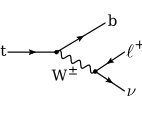
\includegraphics[scale=0.75]{figures/theory/t_decay.pdf}}\hspace{0.15\textwidth}
\subfloat[\label{fig:theory-top-whel-angle}]{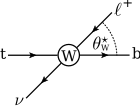
\includegraphics[scale=0.75]{figures/theory/whel.pdf}}
}

Potential scenarios of spin orientations at the $\mathrm{Wtb}$~vertex are presented in Fig.~\ref{fig:theory-top-whel-states} for longitudinal~($H=0$), left-handed~($H=-1$), and right-handed~($H=+1$) $\mathrm{W}$~bosons in the top quark rest frame. In the last scenario the conservation of angular momentum forces the $\mathrm{b}$~quark to be right-handed. This is however suppressed by the electroweak \gls{va} coupling structure leading to a nearly vanishing probability at \gls{lo}. It would vanish entirely for massless $\mathrm{b}$~quarks since then the $\mathrm{b}$~quark helicity would be equal to its chirality~\cite{Bernreuther:2008ju}. The expected distributions per helicity state as a function of $\cos\theta^\star_\mathrm{W}$ are shown in Fig.~\ref{fig:theory-whel-distributions} together with the \gls{nnlo} \gls{sm} expectation of $\mathrm{F}_\mathrm{L}=0.311\pm0.005$, $\mathrm{F}_\mathrm{R}=0.0017\pm0.0001$, and $\mathrm{F}_{0}=0.687\pm0.005$~\cite{Czarnecki:2010gb}. The non-zero but small right-handed helicity fraction arises from the non-zero mass of the $\mathrm{b}$~quark and from the considered corrections beyond \gls{lo} to the vertices.
 
\myfigure{\label{fig:theory-top-whel-states}Scenarios of spin orientations at the $\mathrm{Wtb}$~vertex in the top quark rest frame. The right-handed $\mathrm{W}$~boson helicity~($H=+1$) is suppressed by the electroweak \gls{va} coupling structure which does not allow the right-handed $\mathrm{b}$~quark~(marked in red) to interact.}{
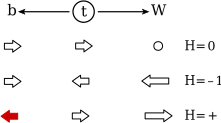
\includegraphics[scale=0.75]{figures/theory/whel_spins.pdf}
}
 
\myfigure{\label{fig:theory-whel-distributions}Distributions of the helicity angle for various W boson helicity scenarios. The \gls{sm} expectation at \gls{nnlo} is taken from Ref.~\cite{Czarnecki:2010gb}.}{
\includegraphics[width=0.6\textwidth]{figures/theory/whel_fractions.pdf}
}

For a general analysis of the top quark spin one introduces the so-called ``spin-analyzing power'', $\alpha_{X}\in[-1;\,1]$\,, of the decay product $X=\ell,\nu,\mathrm{W},\mathrm{b}$~\cite{AguilarSaavedra:2010nx}. It denotes the fraction of instances when the top quark spin is aligned along the momentum of the spin analyzer in the top quark rest frame. The calculated spin-analyzing powers at \gls{lo} and \gls{nlo} in the \gls{sm} are listed in Tab.~\ref{tab:theory-spin-powers}. Additionally, the spin-analyzing powers for $X=\mathrm{q}/\mathrm{q}^\prime$ for $\mathrm{W}\to \mathrm{q}\mathrm{q}^\prime$ decays are provided where $\mathrm{q}$ ($\mathrm{q}^\prime$) denotes all up-type (down-type) quarks respectively. However, studying the top quark spin in those decays is experimentally very challenging since the original quark flavor of a jet and its origin in case of additional final state radiation are difficult to infer. The spin-analyzing powers flip their sign $\alpha_{X}=-\alpha_{\bar{X}}$ in the case of top antiquark decays for the corresponding particle or antiparticle. This holds also in \gls{bsm} scenarios inducing \gls{cp}-violation in the top quark sector.

\mytable{\label{tab:theory-spin-powers}Spin-analyzing power per top quark decay product. The values are taken from Ref.~\cite{AguilarSaavedra:2010nx} and references therein.}{
\begin{tabular}{@{}l  r@{.}l c r@{.}l@{} }
\toprule
Decay product $X$ \hspace{0.4cm}          &  \multicolumn{5}{c@{}}{spin-analyzing power $\alpha_{X}$} \\
\cmidrule{2-6}
& \multicolumn{2}{c}{\gls{lo}}      && \multicolumn{2}{c}{\gls{nlo}} \\
\midrule
$\ell^{\rmplus}$            & \hspace{0.4cm}1&00\hspace{0.4cm}                  && \hspace{0.3cm}0&998 \\
$\nu$                       & -0&32                     && -0&33 \\
$\bar{\mathrm{q}}^\prime$ (down-type)   & 1&00          && 0&93 \\
$\mathrm{q}$~(up-type)      & -0&32                     && -0&31 \\
$\mathrm{b}$                & -0&41                     && -0&39 \\
$\mathrm{W}^{\rmplus}$      & 0&41                      && 0&39 \\
\bottomrule
\end{tabular}
}

The charged lepton is a nearly perfect spin analyzer for studying the top quark polarization. Its spin-analyzing power is even larger than that of its mother particle, the $\mathrm{W}$~boson, due to constructive (destructive) interference of the longitudinal and left-handed $\mathrm{W}$~boson helicity states in cases when the lepton is aligned (antialigned) with the top quark spin, respectively~\cite{Bernreuther:2008ju}. Simplified sketches of various spin orientations for longitudinal and left-handed $\mathrm{W}$~boson helicities are shown in Fig.~\ref{fig:theory-top-spin-orientations} demonstrating that the momentum of the charged antilepton in the top quark rest frame tends to be aligned along the top quark spin. Scenarios with antialigned lepton momentum with respect to the top quark spin~(Figs.~\ref{fig:theory-top-spin-orientations-long-suppressed} and~\ref{fig:theory-top-spin-orientations-left-suppressed}) are suppressed by the \gls{va} coupling structure which does not allow right-handed particles or left-handed antiparticles to interact. Similar diagrams with reversed spin orientations are expected for top antiquarks.

\myfigure{\label{fig:theory-top-spin-orientations}Sketches of various spin orientations in top quark decays for (a,b)~longitudinal and (c,d)~left-handed $\mathrm{W}$~boson helicities. Suppressed spin orientations are marked in red.}{
\subfloat[]{\includegraphics[scale=0.75]{figures/theory/top_spins_long_allowed.pdf}}\hspace{0.15\textwidth}
\subfloat[\label{fig:theory-top-spin-orientations-long-suppressed}]{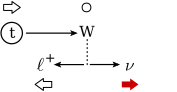
\includegraphics[scale=0.75]{figures/theory/top_spins_long_suppressed.pdf}}\\
\subfloat[]{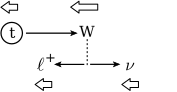
\includegraphics[scale=0.75]{figures/theory/top_spins_left_allowed.pdf}}\hspace{0.15\textwidth}
\subfloat[\label{fig:theory-top-spin-orientations-left-suppressed}]{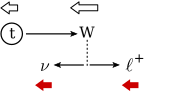
\includegraphics[scale=0.75]{figures/theory/top_spins_left_suppressed.pdf}}
}

%##############################################
\section{Pair production}
%##############################################
\label{sec:theory-ttbar-production}

The dominant mechanism producing top quarks at hadron colliders is top quark pair production through strong interactions via gluon~($gg\to\ttbar$) or quark fusion~($\mathrm{q}\bar{\mathrm{q}}\to\ttbar$). Figure~\ref{fig:theory-feynman-ttbar} shows the corresponding Feynman diagrams at \gls{lo}. Especially the production channel via gluon fusion leads to a large cross section at the \gls{lhc} compared to the Tevatron because of the steeply increasing gluon \gls{pdf} towards smaller momentum fractions. The $gg\to\ttbar$ channel contributes approximately $80\range90\%$ to the total \ttbar production cross section in the \gls{lhc} \acrlong{cm} energy regime of $7\range14~\TeV$~\cite{Olive:2016xmw}. The theoretical \ttbar cross sections in pp collisions at \acrlong{cm} energies of $8$ and $13~\TeV$, relevant for this thesis are listed in Tab.~\ref{tab:theory-ttbar-xsecs}. Those have been calculated at \gls{nnlo}+NNLL accuracy using the \textsc{Top++}\,2.0 program~\cite{Czakon:2011xx,Czakon:2013goa} assuming a top quark mass of $172.5~\GeV$. The \gls{pdf} uncertainty includes also the uncertainty on \as.

\myfigure{\label{fig:theory-feynman-ttbar}Feynman diagrams of \ttbar production at \gls{lo}: (a)~quark fusion; (b,c)~gluon fusion.}{
\subfloat[]{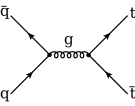
\includegraphics[scale=0.75]{figures/theory/qq2tt_1.pdf}}\hspace{0.03\textwidth}
\subfloat[]{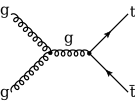
\includegraphics[scale=0.75]{figures/theory/qq2tt_2.pdf}}\hspace{0.03\textwidth}
\subfloat[]{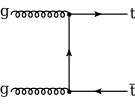
\includegraphics[scale=0.75]{figures/theory/qq2tt_3.pdf}}
}

\mytable{\label{tab:theory-ttbar-xsecs}Top quark pair production cross sections per \acrlong{cm} energy.}{
\begin{tabular}{@{}l r@{.}l@{}l@{$\,\mathrm{(scale)}$}l@{$\,\mathrm{(\gls{pdf})}~\pb$}l@{} }
\toprule
\Acrlong{cm}~energy \hspace{0.3cm}      & \multicolumn{5}{c }{Cross section}     \\
\midrule
$8~\TeV$     & $252$ & $9$ & ${}^{+6.4}_{-8.6}$ & $\pm11.7$ & \\
$13~\TeV$    & $831$ & $8$ & ${}^{+19.8}_{-29.2}$ & $\pm35.6$ & \\
\bottomrule
\end{tabular}
}



%##############################################
\section{Single top quark production}
%##############################################
\label{sec:theory-single-top-production}

Besides producing top quarks in pairs, single top quarks can be produced through electroweak interactions as well. At \gls{lo} one can categorize the production into three main channels depending on the exchanged $\mathrm{W}$~boson and its virtuality, $Q^{2}=-p_{\mu}p^{\mu}$\,. The corresponding Feynman diagrams are presented in Fig.~\ref{fig:theory-feynman-singletop}. Overall, the single-top-quark cross sections are smaller than for pair production due to the electroweak coupling strength $\aw<\as$. Additionally, the requirement of sea quarks~($\mathrm{b}$, $\bar{\mathrm{q}}$) in the initial states whose \glspl{pdf} increase less steeply at low momentum fractions compared to the gluon \gls{pdf} suppresses the cross sections further~(see Fig.~\ref{fig:theory-nnpdf-dist}).

\myfigure{\label{fig:theory-feynman-singletop}Feynman diagrams of electroweak single-top-quark production at \gls{lo} in the 5 flavor scheme.}{
\subfloat[\label{fig:theory-singletop-tch}$t$ channel]{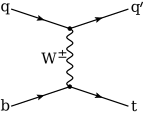
\includegraphics[scale=0.75]{figures/theory/ST_tch.pdf}}\hspace{0.05\textwidth}
\subfloat[\label{fig:theory-singletop-sch}$s$ channel]{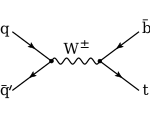
\includegraphics[scale=0.75]{figures/theory/ST_sch.pdf}} \\
\subfloat[\label{fig:theory-singletop-tWch}tW channel]{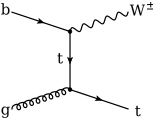
\includegraphics[scale=0.75]{figures/theory/ST_tWch2.pdf}\hspace{0.05\textwidth}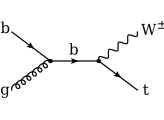
\includegraphics[scale=0.75]{figures/theory/ST_tWch.pdf}}
}

\begin{description}
\item[$\boldsymbol{t}$ channel] The production via $t$-channel~(Fig.~\ref{fig:theory-singletop-tch}) has the highest single top quark cross section in $\mathrm{pp}$ collisions. The virtuality of the $\mathrm{W}$~boson is found to be $Q^2>0$ and hence it is said to be ``space-like''. A characteristic feature of this mode is the production of an additional spectator quark ($\mathrm{q}^\prime$) which recoils against the $\mathrm{W}$~boson and tends therefore to be scattered fairly forward in the \gls{cms} detector~($|\eta|\sim 3$)\,. In this production mode top quarks are produced roughly twice more often than top antiquarks which is a consequence of the up-over-down valence quark composition of the proton. Hence the production ratio, $\sigma(\mathrm{t})/\sigma(\bar{\mathrm{t}})$, is sensitive to the \gls{pdf} of the proton. The ratio depends however on the \acrlong{cm} energy since at higher energies lower momentum fractions are probed at which contributions from the valence quarks become less dominant. 

\item[$\boldsymbol{s}$ channel] Amongst the three main single-top-quark production channels the one with the smallest cross section is the $s$ channel~(Fig.~\ref{fig:theory-singletop-sch}). This is because of the ``time-like'' $\mathrm{W}$~boson ($Q^2<0$) which has to have a large virtuality to produce the heavier top quark. In various \gls{bsm} scenarios however the cross section of this process is expected to increase due to new heavy particles such as $\mathrm{W}^\prime$ or charged Higgs bosons which may even be produced on their mass shell, $p_{\mu}p^{\mu}-m^{2}=0$, and hence occur as a resonance.

\item[tW] The third mode is the production of a single top quark in association with a $\mathrm{W}$~boson~(Fig.~\ref{fig:theory-singletop-tWch}) where the latter can be produced on-shell $Q^2=-m_\mathrm{W}^{2}$\,. It is commonly referred to as ``tW channel''. This process interferes at \gls{nlo} with \ttbar production which complicates its definition. In the \glshere{dr} scheme diagrams with two resonant top quarks are subtracted from the common amplitude whereas in the \glshere{ds} scheme the contribution from \ttbar is locally removed from the cross section~\cite{Tait:1999cf,1126-6708-2009-11-074}. The difference between both schemes lies in the treatment of the interference term which is kept in the \gls{ds} but removed in the \gls{dr}. A new approach has been developed where the \ttbar and tW production and the inference between them are combined into a process with a $\mathrm{W}^{\rmplus}\mathrm{W}^{\rmminus}\,\mathrm{b}\,\bar{\mathrm{b}}+X$ final state~\cite{Cascioli:2013wga} whose simulation is currently being studied~\cite{Jezo:2016ujg}.
\end{description}

The theoretical cross sections of the three single-top-quark production modes in pp collisions for center-of-mass energies of $8$ and $13~\TeV$, relevant for this thesis, are listed in Tab.~\ref{tab:theory-singletop-xsecs}. These have been calculated at \gls{nlo} in \gls{qcd} with the \HATHOR{}\,v$2.1$ program~\cite{Aliev:2010zk,Kant:2014oha} using a top quark mass of $m_\mathrm{t}=172.5~\GeV$ while setting the factorization and renormalization scales to $\mu_\mathrm{R}=\mu_\mathrm{F}=m_\mathrm{t}$. The \gls{pdf} uncertainty includes also the uncertainty on \as.

\mytable{\label{tab:theory-singletop-xsecs}Single top quark cross sections per production mode and \acrlong{cm} energy.}{
\begin{tabular}{@{}l r@{.}l@{}l@{$\,\mathrm{(scale)}$}l@{$\,\mathrm{(\gls{pdf})}~\pb$}l  r@{.}l@{}l@{$\,\mathrm{(scale)}$}l@{$\,\mathrm{(\gls{pdf})}~\pb$}l@{}}
\toprule
Mode\hspace{1cm} & \multicolumn{10}{c }{Cross section / \acrlong{cm} energy}     \\
\cmidrule{2-11}
& \multicolumn{5}{c }{8~TeV} & \multicolumn{5}{c }{13~TeV}  \\
\midrule
$t$ channel     & $84$ & $7$ & ${}^{+2.6}_{-1.7}$ & $\pm2.8$ &   \hspace{0.15cm}   & $217$ & $0$ & ${}^{+6.6}_{-4.6}$ & $\pm6.2$ & \\
tW channel      & $22$ & $4$ & $\pm0.6$ & $\pm1.4$ &      & $71$  & $7$ & $\pm1.8$ & $\pm3.4$ & \\
$s$ channel     & $5$  & $24$ & ${}^{+0.15}_{-0.12}$ & $\pm0.16$ &      & $10$  & $32$ & ${}^{+0.29}_{-0.24}$ & $\pm0.27$ & \\
\bottomrule
\end{tabular}
}

Measurements of single-top-quark cross sections allow to extract a limit on the \gls{ckm} matrix element $\vtb$\,. If one assumes $|\vtd|^2+|\vts|^2\ll|\vtb|^2$ then the $\mathrm{t}\to\mathrm{bW}$ branching ratio can be approximated as

\begin{equation}
\mathcal{B}(\mathrm{t}\to\mathrm{bW})=\frac{|\vtb|^2}{\underbrace{|\vtd|^2+|\vts|^2}_{\ll|\vtb|^2}+|\vtb|^2}\approx 100\%\,.
\end{equation}

Hence, the cross section is independent of the top quark decay vertex and therefore directly proportional to $|f_\mathrm{L}\cdot\vtb|^2$\,. The form factor $f_\mathrm{L}$ is introduced to absorb potential contributions from \gls{bsm} physics that modify the left-handed coupling strength. It is $f_\mathrm{L}^\mathrm{SM}=1$ in the \gls{sm}. A measured single-top-quark cross section can then be used to extract the value of $|f_\mathrm{L}\vtb|$ as

\begin{equation}
|f_\mathrm{L}\vtb|=\sqrt{\frac{\sigma_\mathrm{measured}}{\sigma_\mathrm{theory}}}\,.
\end{equation}

It should be noted that for this interpretation of single-top-quark cross sections, no assumptions on the number of quark generations and subsequently no unitarity of the \gls{ckm} matrix is required.



%##############################################
\section{Polarization in \textit{t}-channel single-top-quark production}
%##############################################
\label{sec:theory-t-channel-polarization}

The \gls{sm} predicts that top quarks are produced highly polarized via $t$~channel since there are only electroweak interactions with a \gls{va} coupling structure involved at \gls{lo}~\cite{Bernreuther:2008ju}. New \gls{bsm} physics models may however lead to a depolarization by altering the coupling structure effectively through new production vertices and/or higher order corrections. The differential cross section as a function of the polarization angle can be parametrized as

\begin{equation}
\frac{\mathrm{d}\sigma}{\sigma\cdot\mathrm{d}\cos\theta^\star_{X}}=\frac{1}{2}\,\Big(1+\mathrm{P}_\mathrm{t}\cdot\alpha_{X}\cdot\cos\theta^\star_{X}\Big)\,,
\end{equation}

where $\mathrm{P}_\mathrm{t}$ denotes the polarization along a given axis and $\alpha_{X}$ the spin-analyzing power with respect to the decay product $X$. The polarization angle

\begin{equation}
\cos\theta^\star_{X}=\frac{\vec{s}_\mathrm{t}\cdot \vec{p}_{X}^\scriptn{\mathrm{(t)}}}{\big|\vec{s}_\mathrm{t}\big|\cdot\big|\vec{p}_{X}^\scriptn{\mathrm{(t)}}\big|}
\end{equation}

is calculated between the spin analyzer $X$ in the top quark rest frame and a suitable spin quantization axis $\vec{s}_\mathrm{t}$. A potential spin axis is given in the helicity basis where the top quark momentum in the partonic \acrlong{cm} system is chosen, $\vec{s}_\mathrm{t}^\scriptn{\,\mathrm{hel.}}=\vec{p}_\mathrm{t}^\scriptn{\mathrm{(tq)}}$. However, this system cannot be reconstructed unambiguously beyond \gls{lo} when additional \glshere{isr} or \glshere{fsr} occurs. An alternative axis is motivated in Fig.~\ref{fig:theory-t-channel-prod-decay} where exemplary spin orientations in the top quark rest frame for $t$-channel production and decay are sketched. There exists a symmetry between the down-type spectator quark on the production side~($\mathrm{q}^\prime$) and the charged antilepton on the decay side~($\ell^{\rmplus}$) leading to a correlation between their momentum directions and the intermediate top quark spin. This suggests to take the spectator quark momentum in the top quark rest frame as the spin quantization axis, $\vec{s}_\mathrm{t}=\vec{p}_{\mathrm{q}^\prime}^\scriptn{\mathrm{(t)}}$\,. At \gls{lo}, this axis would coincide with the axis in helicity basis since the top quark and the spectator quark are back-to-back in the \acrlong{cm} system~\cite{Schwienhorst:2010je}. A high degree of polarization can therefore be expected when quantizing the top quark spin along the spectator quark momentum. This is further motivated by the fact that the charged lepton is a nearly perfect spin analyzer and thus the down-type spectator quark is a good spin analyzer as well because of the depicted symmetry. Higher-order corrections however dilute this symmetry somewhat as also expected from Tab.~\ref{tab:theory-spin-powers} where a slightly lower spin-analyzing power for the down-type quark compared to the charge lepton is expected at \gls{nlo}. 

\myfigure{\label{fig:theory-t-channel-prod-decay}Sketch of spin orientations in $t$-channel single-top-quark production and decay. The figure has been inspired from Ref.~\cite{Schwienhorst:2010je}.}{
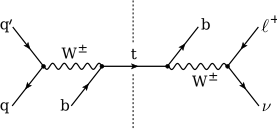
\includegraphics[scale=0.75]{figures/theory/t-channel-prod-decay.pdf}
}

A crucial ingredient which is however missing in this argumentation is the fact that the spectator quark has to be of down-type flavor for obtaining a high polarization. This is  true in about $80\%$ for $t$-channel top quark production but only in $31\%$ of all cases for top antiquark production. In such events the down-type quark is found with a probability of $69\%$ in the initial state instead. However, the spectator quark is only mildly deflected after recoiling against the $\mathrm{W}$~boson. It is therefore still sufficiently close to the direction of the down-type quark momentum which results in a high degree of polarization nonetheless~\cite{Bernreuther:2008ju}.

The expect degrees of polarization for the top quark and top antiquark have been calculated at $7~\TeV$ and are listed in Tab.~\ref{tab:theory-singletop-sm-polarization} at \gls{lo} and \gls{nlo} accuracy. The combined polarization for top quark and antiquark is obtained using a weighted sum with the corresponding cross sections as weights\footnote{The expected single-top-quark cross sections at $7~\TeV$ are $\sigma(\mathrm{t})=41.8^{+1.8}_{-1.5}~\pb$ and $\sigma(\bar{\mathrm{t}})=22.0^{+1.3}_{-1.2}~\pb$. These are calculated with the same setup as used for Tab.~\ref{tab:theory-singletop-xsecs}}. At $8~\TeV$, a similar polarization of $|\mathrm{P}_{\mathrm{t}+\bar{\mathrm{t}}}^\mathrm{8~\TeV}|=0.88$ is expected using simulated events from the \gls{nlo} generator \textsc{Powheg}~\cite{Khachatryan:2015dzz}.

\mytable{\label{tab:theory-singletop-sm-polarization}Expected polarizations of top quarks and top antiquarks in $t$-channel single-top-quark production at $7~\TeV$. The values are taken from Ref.~\cite{Schwienhorst:2010je}.}{
\begin{tabular}{@{}l r@{.}l r@{.}l r@{.}l@{}}
\toprule
            & \multicolumn{2}{c}{$\mathrm{P}_\mathrm{t}^\mathrm{\,7\,\TeV}$} & \multicolumn{2}{c}{$\mathrm{P}_{\bar{\mathrm{t}}}^\mathrm{\,7\,\TeV}$} & \multicolumn{2}{c}{$|\mathrm{P}_{\mathrm{t}+\bar{\mathrm{t}}}^\mathrm{\,7\,\TeV}|$}     \\
\midrule
\gls{lo}    & \hspace{0.5cm}0&99\hspace{0.5cm} & \hspace{0.5cm}-0&93\hspace{0.5cm}       & \hspace{0.5cm}0&95\hspace{0.5cm}          \\
\gls{nlo}   & 0&91                             & -0&86                                   & 0&88          \\
\bottomrule
\end{tabular}
}

The high polarization of the top quark along the spectator quark momentum allows also to extend the $\mathrm{W}$~boson polarization with two additional axes. Figure~\ref{fig:theory-ext-whel} shows the construction procedure. The top quark spin is approximated by the spectator quark momentum. Then the normal and transverse axes are defined as 

\begin{subequations}
\begin{align}
\vec{\mathrm{N}}&=\vec{p}_{\mathrm{q}^\prime}^{\mathrm{(t)}}\times\vec{p}_{\mathrm{W}}^{\mathrm{(t)}}\qquad\text{(normal axis)}\,, \\
\vec{\mathrm{T}}&=\vec{p}_{\mathrm{W}}^{\mathrm{(t)}}\times \vec{\mathrm{N}}\qquad\text{(transverse axis)}\,.
\end{align}
\end{subequations}

\myfigure{\label{fig:theory-ext-whel}Extended $\mathrm{W}$~boson polarization axes in $t$-channel single-top-quark production and decay: $\mathrm{N}=\text{normal axis}$; $\mathrm{T}=\text{transverse axis}$.}{
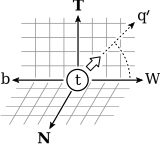
\includegraphics[scale=0.75]{figures/theory/ext_whel.pdf}
}

The differential cross sections as a function of the polarization angles with respect to these new axes take the same functional form as in Eq.~\ref{eq:theory-diff-whel-fractions}. However, the corresponding polarization fractions $\mathrm{F}_\mathrm{L}^\scriptn{\mathrm{N,T}}$, $\mathrm{F}_\mathrm{0}^\scriptn{\mathrm{N,T}}$, and $\mathrm{F}_\mathrm{R}^\scriptn{\mathrm{N,T}}$ are probing different aspects of the coupling structure. In particular, the left- and right-handed polarization along $\vec{\mathrm{N}}$ are sensitive to potential \gls{cp}-violation~\cite{AguilarSaavedra:2010nx}. Since the top quark is not fully polarized along the spectator quark momentum, the  polarization fractions are modified as

\begin{subequations}
\begin{align}
\tilde{\mathrm{F}}_\mathrm{R}^\mathrm{N,T}&=\frac{1+\mathrm{P}_\mathrm{t}}{2}\cdot\mathrm{F}_\mathrm{R}^\mathrm{N,T}+\frac{1-\mathrm{P}_\mathrm{t}}{2}\cdot\mathrm{F}_\mathrm{L}^\mathrm{N,T}, \\
\tilde{\mathrm{F}}_\mathrm{L}^\mathrm{N,T}&=\frac{1+\mathrm{P}_\mathrm{t}}{2}\cdot\mathrm{F}_\mathrm{L}^\mathrm{N,T}+\frac{1-\mathrm{P}_\mathrm{t}}{2}\cdot\mathrm{F}_\mathrm{R}^\mathrm{N,T}, \\
\tilde{\mathrm{F}}_\mathrm{0}^\mathrm{N,T}&=\mathrm{F}_\mathrm{0}^\mathrm{N,T}\,.
\end{align}
\end{subequations}


%##############################################
\section{Flavor schemes}
%##############################################
\label{sec:theory-flavor-schemes}

In single-top-quark production via $t$ channel a $\mathrm{b}$~quark is required in the initial state. There are two approaches called 4 and 5~\glshere{fs} to treat initial state $\mathrm{b}$~quarks in theoretical calculations. They differ in the number of quark flavors considered within the \gls{pdf} of the proton. Figure~\ref{fig:theory-flavorscheme} shows a representative Feynam diagram where in the 4~\gls{fs} the $\mathrm{b}$~quark originates from gluon splitting and is not part of the \gls{pdf}. On the other hand this splitting is resumed into the \gls{pdf} in the 5~\gls{fs} instead.

\myfigure{\label{fig:theory-flavorscheme}Feynman diagram at \gls{lo} for $t$-channel single-top-quark production in 4 and 5~\glsreset{fs}\gls{fs}. The dashed lines denote where the partonic initial state begins.}{
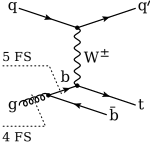
\includegraphics[scale=0.75]{figures/theory/flavorscheme.pdf}
}

Since the $\mathrm{b}$~quark mass of $m_\mathrm{b}\approx4.2~\GeV$ is higher than the mass of the proton ($m_\mathrm{p}\approx1~\GeV$) the 4~\gls{fs} seems more natural at first glance. The $\mathrm{b}$~quark is treated as a heavy quark state that decouples completely from the \as and \gls{pdf} evolutions through renormalization and the DGLAP equation, respectively. However, this approach results in terms proportional to $\log(Q^2/m_\mathrm{b}^2)$ arising from the intermediate $\mathrm{b}$~quark propagator which may prohibit the convergence of perturbative calculations at high momentum transfers $Q$. In this case, such terms together with the $g\to\mathrm{b}\bar{\mathrm{b}}$ splitting function can be absorbed into a \gls{pdf} for the $\mathrm{b}$~quark instead which results in the 4~\gls{fs}~\cite{Maltoni:2012pa}.

Both schemes are valid approaches for calculating observables. The difference between them at fixed order lies in their dependence on the energy scale at which a process is described. The predictions by both schemes will thus converge if calculated at sufficiently high orders. This is demonstrated in Fig.~\ref{fig:theory-t-channel-xsec-fs} where the $t$-channel single-top-quark cross section at $14~\TeV$ as a function of the renormalization and factorization scale is depicted. The dashed curves show the \gls{lo} predictions in 4~and 5~\gls{fs} respectively which are far apart. Their opposite behavior originates from the running of coupling constant \as in the 4~\gls{fs} versus the scale dependence of the $\mathrm{b}$~quark \gls{pdf} in the 5~\gls{fs} as depicted in Fig.~\ref{fig:theory-t-channel-as-fs}. Both approach the \gls{nlo} prediction only at low (large) scales for 4~\gls{fs} (5~\gls{fs}) respectively. On the other hand, the \gls{nlo} predictions start to converge already at a scale choice of about $\mu_\mathrm{R}=\mu_\mathrm{F}= m_\mathrm{t}/2$ for this process.

\myfigure{ In (a): single-top-quark cross section in $t$ channel for top quarks at $14~\TeV$ as a function of the renormalization and factorization scale $\kappa=\mu/m_\mathrm{t}$. Cross sections calculated in 4~and 5~\gls{fs} at \gls{lo} and \gls{nlo} are displayed. The figure is taken from Ref.~\cite{Maltoni:2012pa}. In (b): the relative dependence of the strong coupling constant and the b~quark \gls{pdf} (NNPDF3.0) on the scale $\kappa$ with respect to their values at the Z~boson mass.}{
\subfloat[\label{fig:theory-t-channel-xsec-fs}]{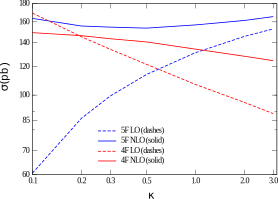
\includegraphics[width=0.555\textwidth]{figures/theory/t-channel-xsec-fs}}
\hspace{0.01\textwidth}\subfloat[\label{fig:theory-t-channel-as-fs}]{\includegraphics[width=0.43\textwidth]{figures/theory/alphaS}}
}

Fixed-order predictions of differential cross sections are also sensitive to the flavor scheme choice. Ratios of the 4~\gls{fs} over the 5~\gls{fs} $t$-channel cross sections at \gls{nlo} as a function of the transverse momentum and pseudo rapidity with respect to the top quark and spectator jet are shown in Fig.~\ref{fig:theory-t-channel-xsec-fs-diff}. The differences between both schemes are found to be around the $10~\%$ level~\cite{Campbell:2009ss}. In particular, the top quark \pt displays here an almost linear increasing ratio.

\myfigure{\label{fig:theory-t-channel-xsec-fs-diff}Ratio of 4~\gls{fs}~($\sigma^{2\to3}$) over 5~\gls{fs}~($\sigma^{2\to2}$) differential \gls{nlo} single-top-quark cross sections in $t$ channel for top quarks at $14~\TeV$ as a function of (a)~the transverse momentum and (b)~the pseudo rapidity of the top quark and light (spectator) jet. The figures are taken from Ref.~\cite{Campbell:2009ss}}{
\subfloat[]{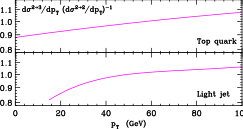
\includegraphics[scale=1]{figures/theory/t-channel-fs-diff-pt.pdf}}\\
\subfloat[]{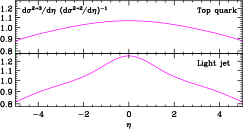
\includegraphics[scale=1]{figures/theory/t-channel-fs-diff-eta.pdf}}
}

%##############################################
\section{Anomalous couplings}
%##############################################
\label{sec:theory-anomalous-couplings}

Direct searches for \gls{bsm} physics can be viewed as a top-down approach. The starting point is marked by a well-defined and usually \gls{uv}-complete \gls{bsm} theory. Experimentally, one is then interested to detect additional events originating from a new process within such a theory. Exemplary models are the \glshere{mssm}~(reviewed in Ref.~\cite{Csaki:1996ks}) or the \glshere{2hdm}~\cite{Branco:2011iw}. Since no signal has been found yet it may be that the energy scale at which a \gls{bsm} process becomes significant is not accessible in direct searches. Nonetheless, potential new particles or interactions will contribute higher-order corrections to processes within the \gls{sm} already at low energies. An example of such a process is the rare $\mathrm{B}^{0}_\mathrm{s}\to\mu^{\rmplus}\mu^{\rmminus}$ decay~\cite{CMS:2014xfa} which can be altered by contributions from e.g. the \gls{mssm}. This motivates a model-independent bottom-up approach where observables of the \gls{sm} are measured with great precision and compared to their expectation. Any deviations can then be interpreted within multiple new theories.

The idea of a bottom-up approach is depicted in Fig.~\ref{fig:theory-t-channel-eff} for some exemplary \gls{uv}-complete theory contributing to single-top-quark production through a new heavy scalar particle $\chi$. If the new particle has a sufficiently high mass it would not be possible to observe it as a new resonance in $s$~channel. However, the shown production of single top quarks would be altered through additional contributions from this new process. At energies $q\ll m_{\chi}$ it would mimic a 4-fermion contact interaction with a simple scalar coupling structure. The \mbox{\gls{sm}+\gls{bsm}}inclusive cross section of this process may still correspond to the one expected from the \gls{sm} alone by fine-tuning the \gls{sm} and \gls{bsm} couplings correspondingly. However, since this new process has a scalar coupling structure it manifests itself as a deviation from the expected \gls{va} coupling structure of the \gls{sm}. Differential cross section measurements and related observables like the top quark polarization can then be used to probe for such anomalous couplings at the production vertex.

\myfigure{\label{fig:theory-t-channel-eff}Feynman diagram of potential \gls{bsm} physics contributing to single-top-quark production via flavor-changing neutral current interaction. At low energies $p\ll m_\chi$ the propagator in (a) can be approximated as an anomalous 4-fermion coupling as shown in~(b).}{
\subfloat[\label{fig:theory-t-channel-chi-uv}$t$~channel]{\parbox{0.35\textwidth}{\centering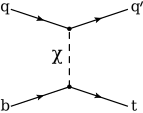
\includegraphics[scale=0.75]{figures/theory/t-channel-chi.pdf}\\$\propto \frac{g^2}{p^2-m^{2}_{\chi}}$}}
\subfloat[\label{fig:theory-t-channel-eff-ir}effective interaction]{\parbox{0.35\textwidth}{\centering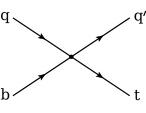
\includegraphics[scale=0.75]{figures/theory/t-channel-contact.pdf}\\$\propto \frac{g^2}{m^{2}_{\chi}}$}}
}

Such deviations from the \gls{sm} coupling structure can be characterized in the framework of effective field theories~(\glsplmark{eft}) in a model-independent manner. Those can be derived using an \glshere{ope} as first proposed in Ref.~\cite{Wilson:1972ee}. Here, products of operators are expanded as

\begin{equation}
{O}_{1}(x_{1})\ldots {O}_{n}(x_{n})=\sum_{i}c_{1\ldots n}^{i}(x_{1},\ldots x_{n})\cdot{O}_{i}^\mathrm{eff}(x_{n})\,,
\end{equation}

where $O_{i}^\mathrm{eff}$ denote effective operators and $c^{i}$ are the so-called Wilson coefficients. The expansion is applicable if $x_{1\ldots n-1}$ are close to $x_n$\,, i.e. only the low energy limit of a \gls{uv}-complete theory is relevant. Otherwise, unitarity can be violated if the energy scale of a process within the \gls{eft} approaches the scale of the concrete \gls{bsm} theory as discussed in Sec.~\ref{sec:theory-observables}. In the example above this would be the case when the momentum transfer $q$ approaches $m_\chi$ at which the \gls{eft} approach becomes invalid.

One can extend the Lagrangian of the \gls{sm}, which contains only operators up to dimension-four, into an effective one as

\begin{equation}
\mathcal{L}^\mathrm{eff}=\mathcal{L}^\mathrm{\gls{sm}}_\mathrm{(4)}+\frac{1}{\Lambda}\sum_{i}c_{i}^\mathrm{(5)}{O}_{i}^\mathrm{(5)}+\frac{1}{\Lambda^{2}}\sum_{i}c_{i}^\mathrm{(6)}{O}_{i}^\mathrm{(6)}+\mathcal{O}\left(\frac{O^\mathrm{(7)}}{\Lambda^3}\right)\,,
\end{equation}

where new effective operators of dimension-five and -six have been added. Those are however suppressed by inverse powers of the new physics scale $\Lambda$. This approach leads to 59 independent operators of dimension-six when requiring gauge invariance and baryon number conservation~\cite{Grzadkowski:2010es}. The only operator of dimension-five is

\begin{equation}
\mathcal{L}^\mathrm{eff.}_\mathrm{(5)}=\frac{1}{\Lambda}c^{ij}_{\nu\nu}\Big({{\mathrm{E}}}^{c}_{\mathrm{L},i}\tilde{\phi}\Big)\Big({\mathrm{E}}_{\mathrm{L},j}\tilde{\phi}\Big)+\mathrm{\gls{hc}},\qquad \tilde{\phi}_{i}=\epsilon_{ij}\phi_{j}
\end{equation}

which can be used to introduce neutrino masses and mixing after electroweak symmetry breaking\footnote{This assumes Majorana neutrinos. The coefficients $c^{ij} v^2/(2\Lambda)$ after symmetry breaking can be interpreted as mass mixing matrix for neutrinos similar to the \gls{ckm} matrix for quarks. The superscript $c$ stands for charge conjugation.}. Only a subset of operators are relevant in the top quark sector~\cite{AguilarSaavedra:2008zc}. In particular, the following operators contribute to the $\mathrm{Wtb}$~vertex


\begin{subequations}\label{eq:theory-eft-lagrangian-operators}
\begin{align}
\mathcal{L}^\mathrm{eff.}_\mathrm{Wtb}&=\mathcal{L}^\mathrm{SM}_\mathrm{Wtb}+\frac{1}{\Lambda^2}\Big(c_{\phi\mathrm{q}}^{33}O_{\phi\mathrm{q}}^{33}+c_{\phi\phi}^{33}O_{\phi\phi}^{33}+c_{\mathrm{dW}}^{33}O_{\mathrm{dW}}^{33}+c_{\mathrm{uW}}^{33}O_{\mathrm{uW}}^{33}\Big)+\mathrm{\gls{hc}}\,,\span\span \\ 
O_{\phi\mathrm{q}}^{33}&=i\Big(\phi^\dagger\omega_{a}\mathrm{D}_\mu\phi\Big)\Big(\bar{\mathrm{Q}}_\mathrm{L}^{3}\gamma^{\mu}\omega^{a}\mathrm{Q}_\mathrm{L}^{3}\Big)\,,&
O_{\phi\phi}^{33}&=i\Big(\tilde{\phi}^\dagger\mathrm{D}_\mu\phi\Big)\Big(\bar{\mathrm{u}}_\mathrm{R}^{3}\gamma^{\mu}\mathrm{d}_\mathrm{R}^{3}\Big)\,,\\
O_{\mathrm{dW}}^{33}&=\Big(\bar{\mathrm{Q}}_\mathrm{L}^{3}\sigma^{\mu\nu}\omega_{a}\mathrm{d}_\mathrm{R}^{3}\Big)\phi\,\mathrm{W}^{a}_{\mu\nu}\,,&
O_{\mathrm{uW}}^{33}&=\Big(\bar{\mathrm{Q}}_\mathrm{L}^{3}\sigma^{\mu\nu}\omega_{a}\mathrm{u}_\mathrm{R}^{3}\Big)\tilde{\phi}\,\mathrm{W}^{a}_{\mu\nu}\,,
\end{align}
\end{subequations}

where $D_\mu$ denotes the covariant derivative~(Eq.~\ref{eq:theory-phi-codev}) and the quark field indices refer to the third generation following the notation of Eqs.~\ref{eq:theory-su2-doublets} and~\ref{eq:theory-su2-singlets}. Anomalous couplings can be introduced after electroweak symmetry breaking which absorb all constant terms including $c_{i}\,v^2/(2\Lambda^2)$\,. One obtains

\begin{align}
\mathcal{L}^\mathrm{eff.}_\mathrm{Wtb}=&-\frac{g}{\sqrt{2}}\bar{\mathrm{b}}\gamma^{\mu}\big(\mathrm{V}_\mathrm{L}\mathrm{P}_\mathrm{L}+\mathrm{V}_\mathrm{R}\mathrm{P}_\mathrm{R}\big)\mathrm{t}\mathrm{W}_\mu^{\rmminus}\nonumber\\
&-\frac{g}{\sqrt{2}}\bar{\mathrm{b}}\frac{i\sigma^{\mu\nu}q_\nu}{m_\mathrm{W}}\big(\mathrm{g}_\mathrm{L}\mathrm{P}_\mathrm{L}+\mathrm{g}_\mathrm{R}\mathrm{P}_\mathrm{R}\big)\mathrm{t}\mathrm{W}_\mu^{\rmminus}+\mathrm{\gls{hc}}\,,\label{eq:theory-wtb-eff-anomcouplings}
\end{align}

where $\mathrm{V}_\mathrm{L,R}$ and $\mathrm{g}_\mathrm{L,R}$ denote the vector- and tensor-like anomalous couplings respectively. In the \gls{sm}~(Eq.~\ref{eq:theory-qqW-int}) there exists only a vector-like, left-handed coupling $\mathrm{V}_\mathrm{L}=\mathrm{V}_\mathrm{tb}$ whereas the other couplings vanish $\mathrm{V}_\mathrm{R}=\mathrm{g}_\mathrm{L}=\mathrm{g}_\mathrm{R}=0$.

Another effective operator relevant for single top quark production is $O_\mathrm{qW}^{ij}$ which is however not associated to the effective Wtb interaction~(Eq.~\ref{eq:theory-eft-lagrangian-operators}). Its contribution can be mostly absorbed by the other operators as

\begin{align}
\mathcal{L}_\mathrm{qW}&=\frac{1}{\Lambda^2}c^{ij}_\mathrm{qW}O_\mathrm{qW}^{ij}=\frac{1}{\Lambda^2}c^{ij}_\mathrm{qW}\Big(\bar{\mathrm{Q}}_{\mathrm{L},i}\gamma^{\mu}\omega_{a}D^\nu\mathrm{Q}_{\mathrm{L},j}\Big)\mathrm{W}_{\mu\nu}^{a}+\mathrm{\gls{hc}}\nonumber\\
&\supset\big(\text{terms }\propto\mathcal{L}_\mathrm{Wtb}^\mathrm{eff.}\big)~+~\frac{g\,\mathrm{Re}(c_\mathrm{qW})}{\Lambda^2}\big(\bar{\mathrm{b}}\gamma^{\mu}\mathrm{P}_\mathrm{L}\mathrm{t}\big)\big(\bar{\mathrm{q}}\gamma_\mu\mathrm{P}_\mathrm{L}\mathrm{q}^\prime\big)+\mathrm{\gls{hc}}\,,\label{eq:theory-4q-eff-anomcouplings}
\end{align}

where however a four-fermion contact interaction term remains~\cite{Bach:2012fb}. This interaction does not contribute to top quark production and decays via a $\mathrm{Wtb}$~vertex directly which is why it is usually not added to Eqs.~\ref{eq:theory-eft-lagrangian-operators} and~\ref{eq:theory-wtb-eff-anomcouplings}. However, the four-fermion vertex cannot be neglected when studying in particular single-top-quark production. Here, it can contribute a $\mathrm{udbt}$~vertex (similar to Fig.~\ref{fig:theory-t-channel-eff-ir}) as an addition to the $\mathrm{Wud}\text{+}\mathrm{Wtb}$~vertices which e.g. occurs in the production via $t$~channel.

To investigate the presence of anomalous couplings in experimental data, various (pseudo) observables are proposed in literature~\cite{AguilarSaavedra:2010nx,Aguilar-Saavedra:2014eqa,Bernreuther:2015yna}. A few of them are the inclusive single-top-quark cross sections, the W~boson helicity fractions~(Sec.~\ref{sec:theory-top-quark-decay}), and the top quark polarization in $t$~channel~(Sec.~\ref{sec:theory-t-channel-polarization}).


%##############################################
\section{Selection of experimental results}
%##############################################
\label{sec:theory-exp-results}

\todo{update to latest results}

To conclude this chapter, a selection of experimental results in the top quark sector are presented. An overview of inclusive \ttbar cross section measurements at \acrlong{cm} energies of 5, 7, 8, and 13~\TeV are shown in Fig.~\ref{fig:theory-lhc-ttbar-xsec} and compared to the theoretical \gls{nnlo}+\gls{nnll} prediction. Measurements of inclusive single-top-quark production in $t$, tW, and $s$~channel at 7, 8, and 13~\TeV are summarized and compared to the theoretical \gls{nlo} predictions in Fig.~\ref{fig:theory-lhc-st-xsec}. These cross section measurements can be used to determine the absolute value of the \gls{ckm} matrix element $\vtb$ as detailed in Sec.~\ref{sec:theory-single-top-production}. The results are presented in Fig.~\ref{fig:theory-lhc-vtb}. The currently most precise estimation of $\vtb$ stems from a combination of $t$-channel single-top-quark cross section measurements at 7 and 8~\TeV by \gls{cms} resulting in $|f_\mathrm{L}\vtb|=0.998\pm0.038\,\mathrm{(exp)}\pm0.016\,\mathrm{(theo)}$. This yields a limit of $|\vtb|>0.92$ at 95\%~\gls{cl} when assuming $f_\mathrm{L}=1$ and $|\vtb|<1$.


\myfigure[p]{Overview of inclusive (a)~\ttbar and (b)~single-top-quark cross section measurements by the \gls{atlas}~and \gls{cms}~collaborations at various \acrlong{cm} energies. The figures are taken from the TopLHC working group~\cite{toplhc}.}{
\subfloat[\label{fig:theory-lhc-ttbar-xsec}]{\includegraphics[width=0.96\textwidth]{figures/theory/tt_curve_sqrts_cms.pdf}}\\
\subfloat[\label{fig:theory-lhc-st-xsec}]{\includegraphics[width=0.9\textwidth]{figures/theory/singletop_allchannels_may2017.pdf}}
}

\myfigure[p]{\label{fig:theory-lhc-vtb}Estimations of the \gls{ckm} matrix element $\vtb$ from single-top-quark cross section measurements. The figure is taken from the TopLHC working group~\cite{toplhc}.}{
\includegraphics[width=0.99\textwidth]{figures/theory/singletop_Vtb_may2017.pdf}
}

The results from measurements of the $\mathrm{W}$~boson helicity fractions are presented in Fig.~\ref{fig:theory-lhc-whel} and compared to their \gls{nnlo} prediction. These have been mostly obtained by analyzing top quark decays in \ttbar events. However, one measurement uses decays of top quarks from $t$-channel single-top-quark production yielding a comparable precision~\cite{Khachatryan:2014vma}.

\myfigure[htbp]{\label{fig:theory-lhc-whel}Overview of $\mathrm{W}$~boson helicity fraction measurements. The figure is taken from the TopLHC working group~\cite{toplhc}.}{
\includegraphics[width=0.95\textwidth]{figures/theory/whelicity_LHC_may2017.pdf}
}

Overall, the various measurements presented here show a good agreement with the \gls{sm} prediction. Since no deviation is observed, limits on the anomalous couplings can be derived. Global fits of the anomalous couplings are however a complicated and computing-intense undertaking. Given a certain point in the coupling hyperspace, multiple observables need to be computed and compared to the results from various measurements while accounting for statistical and systematic uncertainties. A sophisticated fitting framework called \TOPFITTER[format=hyperbf] has been recently developed~\cite{Buckley:2015lku}. The estimated couplings strength per operator contributing to single-top-quark production obtained from various measurements at the \gls{lhc} and the Tevatron are shown in Fig.~\ref{fig:theory-eft-fit}. The results are found to be consistent with the \gls{sm} expectation where those operators vanish.

\myfigure[htbp]{\label{fig:theory-eft-fit}Coupling strength per operator contributing to single-top-quark production. Shown are 95\% confidence intervals. The Wilson coefficient $C_\mathrm{t}$ contains all contributions from four-fermion interactions. The figure is taken from Ref.~\cite{Buckley:2015lku}.}{
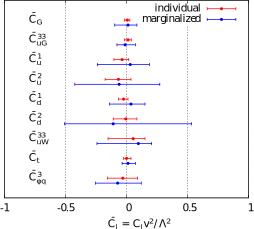
\includegraphics[scale=0.85]{figures/theory/EFT_fit.pdf}
}





%\chapter{Experimental setup}

\section{Large Hadron Collider}

\subsection{Accelerator complex}

\subsection{Experiments}

\section{CMS experiment}

\subsection{Magnet}

\subsection{Tracker}

\subsection{Electromagnetic calorimeter}

\subsection{Hadronic calorimeter}

\subsection{Muon systems}
DT/RPC/CSC

\subsection{Data acquisition}
Trigger/DAQ

\subsection{Operations}
DCS/DSS

\chapter{Reconstruction of physics objects}

%\chapter{Analysis techniques}

\intro{This chapter introduces the necessary toolset to perform the analyses within this thesis. It is organized to follow the common steps of the analyses. First, the generation of simulated events is introduced. Then, details of the top quark reconstruction, the employed multivariate analysis technique, and the template fit is given which are used to estimate the amount of single top quark events within the recorded data. Lastly, the partonic and fiducial objects are defined to which the observed data is unfolded to for comparison with theoretical predictions.}

%##############################################
\section{Event generation}
%##############################################
\label{sec:technique-event-gen}

To compare reconstructed data with theoretical predictions, samples of simulated events are generated from theory and passed through a simulation of the \gls{cms} detector and emulation of its readout. The standard so-called ``FullSimulation'' package~\cite{1742-6596-396-2-022003,1742-6596-664-7-072022} is based on the Geant4 toolkit~\cite{Agostinelli2003250} which provides a detailed simulation of particle trajectories and interactions with the detector material. A fast alternative, the so-called ``FastSimulation'' package, exists within \gls{cms} as well~\cite{fsimRahmat} but has not been used for simulating the detector response in the analyses within this thesis.

The event generation starts with the \glshere{me} of a hard scattering process of interest. \glshere{mc} methods are employed to sample the corresponding cross section integral. The advantage of \gls{mc}-based methods is that the variance of their result decreases as $1/n$ independently of the integral's dimensionality leading to an efficient convergence compared to quadrature-based methods~(e.g. Simpson's rule, Newton-Cotes). A common method to integrate cross sections is given by the \gls{vegas} algorithm~\cite{OHL199913}. It is based on importance sampling where the integral is sampled not uniformly but along an adaptive importance function instead. The resulting sample of events reflects the probability distribution of a process over its phase space. Typically a reweighting is performed in addition such that all events contribute the same probability (e.i. they carry the same absolute weight). 

After obtaining events from the hard interaction, a \glshere{ps} program simulates the hadronization of final state partons. In addition, the radiation of gluons or quarks from initial or final state partons is accounted for as well as contributions from soft secondary interactions, the so-called underlying event, and potential color reconnection effects. A sketch of various parts within an exemplary pp collision event after hadronization is shown in Fig.~\ref{fig:technique-mcevent}. The \gls{ps} simulation is based on Altarelli-Parisi splitting functions~\cite{Altarelli:1977zs} which allow to calculate the probability of soft parton emissions, e.g. $\mathrm{q}\to \mathrm{gq}$. It is convenient to calculate the ``surviving'' probability, the so-called Sudakov factor, that a parton does not branch further below a certain energy scale. During the \gls{ps} simulation a complication arises from potential double counting of soft parton emissions since the simulation of the hard interaction may lead to a soft emission as well which is however already accounted for by the \gls{ps}. These are avoided by applying a \gls{me}-to-\gls{ps} matching scheme which yields a criterion to assign additional emissions to either the simulation of the hard interaction or the \gls{ps} exclusively depending on the event kinematics. A general introduction to parton shower simulation and matching algorithms can be found in Refs.~\cite{Hoche:2014rga,Alwall:2007fs}.


\myfigure{\label{fig:technique-mcevent} A sketch of a generated event from the simulation of the hard interaction and subsequent hadronization through a parton shower. The figure is taken in parts from Ref.~\cite{Hoche:2014rga}.}{
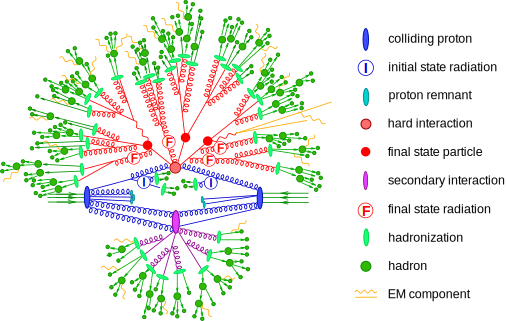
\includegraphics[scale=0.75]{figures/technique/shower.pdf}
}

A brief overview of the programs used for generation and subsequent hadronization of $t$-channel single top quark production is given in the following.

\begin{description}
\item[MadGraph5\_aMC{@}NLO] The \MGAMC program~\cite{Alwall:2014hca} is a merge of the \gls{lo} \MG generator~\cite{Alwall:2011uj} and \AMC into a common framework. It supports the generation of \gls{lo} or \gls{nlo} samples which can be matched to parton showers using the MLM~\cite{Mangano:2006rw} or MC{@}NLO~\cite{Frixione:2002ik} schemes respectively. The latter method produces a certain fraction of events with negative weights (depending on the process) which stem from a subtraction of additional emissions from the \gls{nlo} matrix element to prevent double-counting. 
Multiple samples of events with additional final state partons at matrix element level can also be merged into a combined sample. Here, the overlap with the \gls{ps} is removed through the FxFx merging scheme~\cite{Frederix:2012ps}.

\item[Powheg] The \POWHEG box (versions~1,2)~\cite{Alioli:2010xd} is a program that contains predefined implementations of various processes such as $t$-channel single top quark production~\cite{Alioli:2009je} at \gls{nlo}. It utilizes the so-called \POWHEG method~\cite{Frixione:2007vw} for matching in which the hardest radiation generated from the \gls{me} has priority over subsequent \gls{ps} emissions. This removes the overlap with the \gls{ps} without the generation of negatively weighted events.

\item[CompHEP] The \COMPHEP program (version~4.5)~\cite{Boos:2004kh} can perform calculations of cross sections from Lagrangians at \gls{lo}. In addition, generation of events is also possible such as single top quark production~\cite{Boos:2006af}. Here, an approximation is used by combining events from the $2\to2$ and $2\to3$ processes which reproduces effectively \gls{nlo} corrections.

\item[Tauola] \todo{?}

\item[Pythia] The \PYTHIA program (versions~6,8)~\cite{Sjostrand:2006za,Sjostrand:2014zea} can generate events of various processes at \gls{lo}. It is however famous for its \gls{ps} simulation which can be interfaced with other \gls{lo} and \gls{nlo} event generators to perform subsequent parton showering, hadronization, and the simulation of the underlying event. For hadronization, a phenomenological model is utilized in which one-dimensional strings\footnote{The string model is motivated by the fact that the spatial form of a dipole color field does not extend radially like an \gls{em} field but is instead squeezed to a tube-like form.} connected to partons reflect the color field leading to the creation of additional partons through string branching and finally to the formation of color-neutral singlets.

\item[Herwig++] The \HERWIG program (version~7)~\cite{Bellm:2015jjp} is an \gls{nlo} event generator which is also capable of simulating the showering of partons similar to \PYTHIA. Its hadronization algorithm utilizes a model in which color-connected quarks are spatially kept together in clusters~\cite{Webber:1983if} which is motivated by the ``preconfinement'' of color~\cite{Amati:1979fg}. If the mass of a cluster is sufficiently high it can decay into lighter clusters with a certain probability. In its final step, a cluster decays then into a pair of hadrons.
\end{description}




%##############################################
\section{Top quark reconstruction}
%##############################################

After the reconstruction and selection of analysis objects, a top quark candidate is reconstructed in the presented analyses. Assuming that the top quark decayed leptonically as $\mathrm{t}\to\mathrm{b}\mathrm{W}\to\mathrm{b}\ell\nu$ its energy and momentum is reconstructed by summing the measured 4-momenta of a selected lepton (muon or electron), b-tagged jet, and neutrino candidate. The neutrino candidate itself is reconstructed from the missing transverse energy and the lepton momentum by requiring a W~boson mass constraint of $m_\mathrm{W}=80.4~\GeV$~\cite{Olive:2016xmw} on their invariant mass as

\begin{align}
m_\mathrm{W}^2=\colvec{2}{E_\mathrm{W}}{\vec{p}_\mathrm{W}}^{2}&\overset{!}{=}\left[\colvec{2}{E_{\ell}}{\vec{p}_{\ell}}+\colvec{2}{E_{\nu}}{\vec{p}_{\nu}}\right]^{2}\nonumber\\
&=\underbrace{m_{\ell}^2+m_{\nu}^2}_{\approx 0}+\,2\cdot E_{\ell}\,E_{\nu}-\,2\cdot\colvec{3}{p_{\ell,x}}{p_{\ell,y}}{p_{\ell,z}}\cdot\colvec{3}{p_{\nu,\mathrm{T}}\cdot\cos\phi_{\nu}}{p_{\nu,\mathrm{T}}\cdot\sin\phi_{\nu}}{p_{\nu,z}}. \label{eq:technique-neutrino-pz-eq}
\end{align}

When taking $p_{\nu,\mathrm{T}}$ and $\phi_{\nu}$ from the missing transverse momentum vector $\pvmiss$, this allows to solve for the unknown $p_{\nu,z}$-component of the neutrino candidate momentum. After rearranging, one obtains from Eq.~\ref{eq:technique-neutrino-pz-eq} the quadratic equation

\begin{equation}
0=p_{\nu,z}^2-\frac{2\,\xi\,p_{\ell,z}}{E_{\ell}^{2}-p_{\ell,z}^2}\cdot p_{\nu,z}-\frac{\xi^{2}-E_{\ell}^{2}\,p_{\nu,\mathrm{T}}^2}{E_{\ell}^{2}-p_{\ell,z}^2},\end{equation}

with

\begin{equation}
\xi=\frac{m_\mathrm{W}^2}{2}+p_{\nu,\mathrm{T}}\,p_{\ell,\mathrm{T}}\cdot\cos\big(\phi_\ell-\phi_\nu\big)
\end{equation}

which possesses the solutions

\begin{align}
p_{\nu,z}^{1,2}=\frac{1}{E_{\ell}^{2}-p_{\ell,z}^{2}}\left[\xi\cdot p_{\ell,z}\pm E_{\ell} \sqrt{\xi^2-p_{\nu,\mathrm{T}}^2\big(E_{\ell}^2-p_{\ell,z}^2\big)}~\right]. \label{eq:technique-neutrino-pz}
\end{align}

A detailed derivation and discussion of this result can be found in Ref.~\cite{Chwalek:1416031}. In simulated $t$-channel single-top-quark events this procedure leads to two real solutions for the neutrino $p_{\nu,z}$-component in about 65\% of all events that passed the selection. The difference of the two real solutions with respect to the true neutrino $p_{z}$ at parton level is displayed in Fig.~\ref{fig:technique-neutrino-reco}. 

\myfigure{\label{fig:technique-neutrino-reco}Differences of the reconstructed neutrino $p_{z}$ with respect to the neutrino $p_{z}$ at parton level in cases of real and complex solutions. The distributions have been generated using \POWHEG interfaced with \TAUOLA and \PYTHIA8.}{
\includegraphics[width=0.52\textwidth]{figures/technique/neutrino_match_dpz.pdf}
}

The plot demonstrates that choosing the solution which has the smallest absolute $|p_{\nu,z}|$ yields on average a neutrino $p_{z}$ which is closest to the true neutrino $p_{z}$. If the discriminant in Eq.~\ref{eq:technique-neutrino-pz} becomes negative the solutions are complex. This happens in about 35\% of events and occurs mostly due to the finite \met resolution whereas the negligence of the W~boson mass width and resolution of the lepton momentum are minor effects. The imaginary part of the solutions is removed by requiring that the discriminant vanishes

\begin{equation}
0\overset{!}{=}\xi^2-p_{\nu,\mathrm{T}}^2\big(E_{\ell}^2-p_{\ell,z}^2\big)~
\Rightarrow~ p_{\nu,z}=\frac{\xi\cdot p_{\ell,z}}{E_{\ell}^{2}-p_{\ell,z}^{2}}
\end{equation}

which is equal to setting the transverse W~boson mass $\mtw$ to the W~boson mass itself

\begin{align}
m_\mathrm{W}^2\overset{!}{=}\mtw^2&=(p_{\ell,\mathrm{T}}+p_{\nu,\mathrm{T}})^2-(p_{\ell,x}+p_{\nu,x})^{2}-(p_{\ell,y}+p_{\nu,y})^{2}\nonumber\\
&=2\,p_{\ell,\mathrm{T}}^2\,p_{\nu,\mathrm{T}}^2\cdot\Big[1-\cos\big(\phi_\ell-\phi_\nu\big)\Big].
\end{align}

Then, the $p_{\nu,x}$ and $p_{\nu,x}$ components are varied and the transverse momentum which minimizes the distance $|\vec{p}_{\nu,\mathrm{T}}-\pvmiss|$ with respect to the measured missing transverse momentum vector is taken as the result. 

After finding a solution for the unknown neutrino $p_{z}$ component, a top quark candidate can be constructed from the 4-momenta of the lepton, b-tagged jet, and neutrino candidate. Shape comparisons of the top quark mass and pseudorapidity for the two neutrino solution cases are presented in Fig~\ref{fig:technique-top-reco}. In the case that only a complex solution has been found an improved reconstructed top quark mass resolution is achieved. Similarly, the pseudorapidity of the top quark candidate demonstrates an improved reproduction of the corresponding observable at parton level as well.

\myfigure{\label{fig:technique-top-reco} Shape differences in the reconstructed top quark (a)~mass and (b)~pseudorapidity for cases with real neutrino $p_{z}$ solutions where the one with the smallest $|p_{z}|$ is picked or only a complex solution. The distributions have been generated using \POWHEG interfaced with \TAUOLA and \PYTHIA8.}{
\subfloat[]{\includegraphics[width=0.48\textwidth]{figures/technique/top_match_mass.pdf}}\hspace{0.03\textwidth}
\subfloat[]{\includegraphics[width=0.48\textwidth]{figures/technique/top_match_eta.pdf}}
}

\todo{top quark matching performance
(top pT/eta as function of b-tag in acceptance after selection, b-quark within dR, top within dR)}

%##############################################
\section{Boosted Decision Trees}
%##############################################

The $t$-channel single-top-quark signal region, defined by one isolated lepton, 2~jets (where one is b-tagged), and significant \met, is found to be still largely contaminated by events from background processes after the event selection. The \glshere{sb} yield ratios are about 13\% and 14\% in analyses at 8~and 13~TeV, respectively~\cite{Khachatryan:2014iya,Sirunyan:2016cdg}\todo{update TOP-16-003 when accepted by PRL}. The majority of background events stems from \wjets, \ttbar, and multijet production whereas contributions from single top quark tW and $s$-channel, Drell-Yan, and diboson production are minor. The small \gls{sb} ratio motivates the usages \glshere{mva} techniques. In this thesis, \glsplhere{bdt} are employed for event classification as implemented in the \gls[]{tmva} framework~\cite{Hocker:2007ht}. They are based on a set of decision trees where each yields a binary output depending on whether an event is signal- or background-like. Their training and how the single decision tree outputs are combined into a one-dimensional discriminant are detailed in the following.

An exemplary decision tree is presented in Fig.~\ref{fig:technique-decisiontree} where sequential selections on observables $x_{i}$ are applied such that the leaf nodes contain either a majority of signal or background events. Such a tree is build from samples of simulated events for which the desired classification is a priori known~(``superivsed learning'').

\myfigure{\label{fig:technique-decisiontree} A sketch of a decision tree.}{
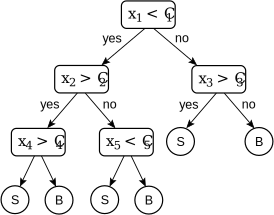
\includegraphics[scale=0.75]{figures/technique/decision_tree.pdf}
}

By maximizing the separation between the signal and background distributions per node the optimal observable $x_{i}$ and working point $C_{i}$  are found. In the analyses, the separation is calculated as the cross entropy 

\begin{align}
H&=-p\cdot\ln(p)-(1-p)\cdot\ln(1-p)\\ p_{i}&=\frac{\int_{C_{i}}^{\infty} N_\mathrm{sig.}(x_{i})\,\mathrm{d}x_{i}}{\int_{C_{i}}^{\infty} N_\mathrm{sig.}(x_{i})+N_\mathrm{bkg.}(x_{i})\,\mathrm{d}x_{i}}\\
\Rightarrow &~\{x_{i},\,C_{i}\}=\max\Big(H\,\big|~x_{i},\,C_{i}\Big)
\end{align}

where $p$ denotes the achieved purity of a selection $x_{i}>C_{i}$. Other common measures of separation are the misclassification error or the so-called ``Gini'' index~\cite{Gini}. The separation measures are constructed to be symmetric when swapping the signal and background classes since obtaining a background leaf with high purity is of equal importance. A node is not split if it contains less than a predefined minimum number of events to ensure that the decisions per node and the binary outputs per leaf are statistically significant. This also mitigates a potential ``overtraining'' of a decision tree which occurs when statistical fluctuations are learned instead of the underlying physical distributions due to the finite statistics of the training sample. Additional caution is required when using a sample which contains a portion of negatively weighted events~(e.g. generated with \MGAMC). In such a case, a tree may be trained incorrectly if a large fraction of negatively weighted events are selected in one of the nodes since the distributions of observables can contain regions with unphysical yields. To tweak the cancellation of negatively weighted events the minimum number of events can be increased further beyond the statistical motivated threshold one would choose when training only on a sample of purely positively weighted events. In addition, the working point values per observable which are analyzed to find the optimal node splitting can be preset which prevents that a decision becomes sensitive to single events close to the selection border.

Single decision trees can still be perceptible to statistical fluctuation leading to misclassification errors when given a statistically-independent test sample. This is mitigated by training multiply decision trees with binary outputs $h_{i}\in\{-1,1\}$ that are then combined into a pseudo-continuous discriminant using a majority vote as

\begin{equation}
M(\vec{x})=\sum_{i}^{N_\mathrm{trees}}~w_{i}\cdot h_{i}\,(\vec{x};\,\vec{C}_{i}).\label{eq:technique-majority-vote}
\end{equation}

Here, each decision tree output is multiplied by a so-called boosting weight $w_{i}$. This way of combining multiple decision trees has another advantage. It has been shown that the majority vote can yield a classifier with high accuracy by applying a ``boosting'' procedure. Such a ``strong learner'' can already be obtained if the individual decision trees are just ``weak learners'' which means that they have only a low classification accuracy~\cite{Schapire1990,FREUND1995256}. The decision trees can therefore be kept very shallow, e.g. only two or three layers of selections, which also improves their robustness against overtraining. A boosting procedure accounts then for the individual accuracy per tree by adjusting its weight accordingly in the majority vote which results into a strong learner.

The two boosting procedures employed in this thesis are the adaptive boosting, \ADABOOST~\cite{FREUND1997119}, and \GRADIENTBOOST~\cite{Friedman00greedyfunction} algorithms. In the \ADABOOST algorithm, decision trees are trained iteratively. At each step, a single decision tree is trained and the misclassified events are identified. Their weight is then increased in the training of subsequent trees by the boosting weight

\begin{equation}
\alpha_{n+1}=\left(\frac{1-\epsilon_{n}}{\epsilon_{n}}\right)^\beta
\end{equation}

where $\epsilon_{i}$ denotes the misclassification rate of the current tree $n$ and $\beta$ is a configurable learning rate. The corresponding weight in Eq.~\ref{eq:technique-majority-vote} is then given by $w_{i}=\ln\alpha_{i}$. Typically, a slow learning rate of $\beta\leq0.5$ is chosen to allow for more boosting steps. It can be shown that the \ADABOOST algorithm is equivalent to the minimization of the exponential loss function $L(M,y)=\exp(-M(\vec{x})\,y)$ where $y$ denotes the true classification of events~\cite{Hocker:2007ht}. If the loss function is instead changed to 

\begin{equation}
L(M,y)=\ln\left(1+e^{-2\,M(\vec{x})\,y}\right)
\end{equation}

the \GRADIENTBOOST algorithm is obtained. Its loss function is more robust in the presence of outliers and noise events for which the \ADABOOST algorithm may degrade. The algorithm commences by iteratively minimizing the loss function with respect to the weights and decision tree parameters in $M$ using the method of gradient decent. During the minimization steps, the output of the majority vote will gradually tend towards $y$ because misclassified events result in large gradients of the loss function. Similar to the \ADABOOST algorithm, an increased performance is obtained when decreasing the learning rate controlling the boosting weights which is called ``shrinkage'' here. In this thesis, both boosting algorithms have been tested to validate their performances with respect to each other. Only negligible differences in their discrimination power have been found after optimizing their training parameters.

The discrimination power of a trained \gls{bdt} is assessed by analyzing the \glshere{roc} curve. Exemplary \gls{roc} curves are presented in Fig.~\ref{fig:technique-bdt-rocs}. The \gls[]{auc} values denote the area under the \gls{roc} curve with respect to random guessing. Here, the \gls{roc} curves of a \gls{bdt} trained to discriminate $t$-channel single-top-quark events against \wjets and \ttbar background events is compared to the pseudorapidity of the untagged light jet and to the reconstructed top quark mass difference. An \gls{auc} of about $32\%$ is achieved with the trained \gls{bdt} which outperforms the other two typical event observables for separating $t$-channel events from background processes. The exact setup of the \gls{bdt} shown here will be discussed in Sec.~\ref{sec:diff13-bdt} together with the corresponding analysis.

\myfigure{\label{fig:technique-bdt-rocs}Comparison of \gls{roc} curves for separating $t$-channel single-top-quark events from background events (\wjets, \ttbar) using: random guessing; a trained \gls{bdt} discriminant; the pseudorapidity of the untagged light jet ($\jprime$); the difference of the reconstructed top quark mass with respect to the nominal mass, $\Delta m_\mathrm{top}=m_\mathrm{top}-172.5~\GeV$.}{
\includegraphics[width=0.5\textwidth]{figures/technique/rocs.pdf}
}


%##############################################
\section{Template-based fitting}
%##############################################

In the analyses, the amount of signal and background events is estimated from data using template-based \glshere{ml} fits. For an observable to be fitted, histograms of simulated events act as templates which reflect the expected distributions of events per process. The likelihood that the observed distribution in data is a realization of the expectation from simulation can then be expressed as

\begin{equation}
\mathsf{L}_\mathrm{Poi.}=\prod_{i}^\mathrm{bins}~\frac{p_{i}^{\,d_{i}}\cdot e^{-p_{i}}}{d_{i}!},\qquad p_{i}=\beta^{\mathrm{(sig.)}}\cdot t^{\mathrm{(sig.)}}_{i}+\sum_{j}^\mathrm{bkgs.}~\beta^{(j)}\cdot t^{(j)}_{i}. \label{eq:technique-likelihood}
\end{equation}

The amount of observed data events $d_{i}$ per bin $i$ is modeled to follow a Poisson distribution with an expected event yield $p_{i}$. The expected yields are obtained by summing the respective contributions of the signal and background templates $t^\scriptn{(X)}_{i}$ per process $X$. The normalization per process is controlled through scale factors $\beta^\scriptn{\mathrm{(X)}}$. These are then estimated through the fit from data by maximizing the likelihood. The signal scale factor is also referred to as signal ``strength'' whereas the background scale factors are sometimes called nuisance parameters because their estimation is of less importance. Technically, the \THETA framework~\cite{theta} is employed for template-based fitting where for convenience and numerical stability reasons the negative logarithm of the likelihood

\begin{equation}
-\ln\Big(\mathsf{L}_\mathrm{Poi.}\big(\vec{\beta}\big)\Big)=-\sum_{i}^\mathrm{bins}~\Big[\,d_{i}\ln p_{i}\big(\vec{\beta}\big)-p_{i}\big(\vec{\beta}\big)\Big]+\mathrm{const.}
\end{equation}

is minimized which is however equivalent to maximizing Eq.~\ref{eq:technique-likelihood} with respect to the scale factors. Since the templates are normalized to their corresponding \gls{sm} cross sections times the integrated luminosity, an estimated scale factor can be directly translated into a corresponding cross section as

\begin{align}
\hat{\sigma}_\mathrm{sig.}&=\frac{\hat{N}_\mathrm{sig.}}{A\cdot\epsilon\cdot{\textstyle{\int}L}}~,\quad
\hat{N}_\mathrm{sig.}=\hat{\beta}_\mathrm{sig.}\cdot N_\mathrm{exp.}=\hat{\beta}_\mathrm{sig.}\cdot\underbrace{\sigma_\mathrm{\gls{sm}}\cdot\textstyle{\int}L}_\mathrm{normalization}\cdot \overbrace{A \cdot \epsilon}^\mathrm{selection}\nonumber\\
&=\hat{\beta}_\mathrm{sig.}\cdot\sigma_\mathrm{\gls{sm}}
\end{align}

where $A$ denotes the acceptance and $\epsilon$ the efficiency of the event selection which are intrinsically estimated through the simulated samples. For the background scale factors additional constraints are applied by adding log-normal priors to the likelihood as

\begin{equation}
-\ln\Big(\mathsf{L}_\mathrm{bkgs.}\Big)=\sum_{j}^\mathrm{bkgs.}~\frac{1}{2}\cdot\left(\frac{\ln\,\beta^{(j)}}{\delta^{(j)}}\right)^{2}.
\end{equation}

These additional constraints with uncertainties $\delta$ reflect a priori believes of the background contributions in the signal phase space where the fit is carried out. They are motivated by the fact that the selected analysis phase space is usually only optimized to measure the signal process accurately but not the background contributions. Here, log-normal distributions are explicitly preferred to model the constraints over Gaussian distributions because in the case of large uncertainties log-normal distributions will not be biased when requiring that the scale factors are always positive. For Gaussian distributions with large widths, such a truncation shifts the mean of the distribution which then biases the fit result.

In the fit, an extra uncertainty is considered to account for the limited accuracy of the predicted event yields per bin due to the finite statistics of the simulated event samples. A method proposed by R. Barlow and C. Beeston~(\gls[]{bb})~\cite{Barlow:1993dm} is to model this uncertainty by adding additional nuisance parameters $\nu_{ij}$ for each bin $i$ and process $j$ which modifies the predicted yields as $p_{i}^\prime=\sum_{j}\nu_{ij}\cdot p_{ij}$. These so-called \gls{bb} parameters are constrained in the likelihood to reflect the uncertainties of the sample statistics. This approach however increases the complexity of the fit since many more parameters have to be estimated in addition to the signal and background scale factors. The number of free parameters is reduced in the Barlow-Beeston lite method~\cite{Conway:2011in} where the uncertainties per bins are grouped and describe by only a single nuisance parameter. A further, technical simplification can be achieved when using numerical minimization algorithms for fitting. Here, it is computationally advantageous to only maximize the likelihood with respect to the scale factors while adjusting the \gls{bb} parameters adaptively to cover the remaining difference between prediction and data per bin. This approach is also implemented in the employed \THETA framework.



%##############################################
\section{Parton and particle level observables}
%##############################################

Cross sections can be measured not only inclusively but also differentially in intervals of an observable. Differential cross sections offer the means to perform in-deep comparisons of data with theoretical predictions. The result of such measurements allows to assess the modeling and validity of event generators and analytical calculations. Furthermore, as detailed in Ch.~\ref{ch:top}, some differential cross sections can be sensitive to the coupling structure of a process and can thus be interpreted in potential \gls{bsm} scenarios as well.

A proper comparison of differential cross sections can only be achieved if the corresponding observable is well-defined and identical across generators and analytical calculations. There are two ``levels'' at which physics objects of a process and related observables are typically defined. These are presented in Fig~\ref{fig:technique-parton-particle}.

\myfigure{\label{fig:technique-parton-particle}A sketch of parton and particle level objects in $t$-channel single-top-quark production.}{
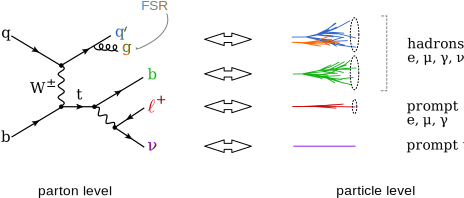
\includegraphics[scale=0.75]{figures/technique/fiducial.pdf}
}

The parton level corresponds to the intermediate and final state particles within a Feynman diagram. In event generators, these particles are produced as the hard interaction before the event is handed to a parton shower program where result of the hadronization and various other effects~(see Fig.~\ref{fig:technique-mcevent}) are simulated. The partonic top quark is defined to be on-shell while accounting for \gls{qcd}/\gls{qed} radiations and the intrinsic $k_\mathrm{T}$ of initial state partons which may boost the event. Prompt leptons which originate from the W~boson decay are defined in the same manner. About 15\% of the final state electrons or muons originate from a leptonically decaying tau lepton, these leptons are included into the definition as well. The fraction depends on the \pt threshold of the muon or electron as depicted in Fig.~\ref{fig:technique-parton-muon}. When selection electron or muons with a $\pt$ of at least $20~\GeV$ this the fraction of leptonically decaying tau leptons entering the selected phase space reduces to 6\%.


The spectator quark may radiate a gluon as shown exemplary. At \gls{nlo}, this can lead to an ambiguity if it is accounted

ambigous at NLO, 4/5FS because of 2nd b-quark

\textit{''The unfortunate truth is that most of the event record is intended
for generator debugging rather than physics interpretation''}~\cite{Buckley:2010ar}.



\myfigure{\label{fig:technique-parton-muon}Distributions of the (a)~transverse momentum and (b)~pseudorapidity of the final state lepton produced in $t$-channel single top quark production at $13~\TeV$. The lines represent various decays of W~bosons into either direct muons/taus or into muons via intermediate tau decays. The distributions have been generated using \POWHEG interfaced with \TAUOLA and \PYTHIA8.}{
\subfloat[]{\includegraphics[width=0.48\textwidth]{figures/technique/lepton_pt.pdf}}\hspace{0.03\textwidth}
\subfloat[]{\includegraphics[width=0.48\textwidth]{figures/technique/lepton_eta.pdf}}
}
\myfigure{\label{fig:technique-parton-cosTheta}Distributions of the polarization angle for $t$-channel single top quark production at $13~\TeV$: (a)~inclusive distribution; (b)~only events with $\pt(\mu)>20~\GeV$. The lines represent various decays of W~bosons into either direct muons/taus or into muons via intermediate tau decays. The distributions have been generated using \POWHEG interfaced with \TAUOLA and \PYTHIA8.}{
\subfloat[]{\includegraphics[width=0.48\textwidth]{figures/technique/cosTheta.pdf}}\hspace{0.03\textwidth}
\subfloat[]{\includegraphics[width=0.48\textwidth]{figures/technique/cosTheta_lpt20.pdf}}
}

dressed leptons (cone algorithms associates photons to leptons but does not cluster close leptons), tau decays, jet clustering (no neutrinos/leptons), b-tagging, rivet, drop of cosTheta at 1 through lepton pT cut



%##############################################
\section{Unfolding}
%##############################################

Unfolding in \gls{hep} is a procedure which attempts to infer a distribution at parton or particle level from data. The idea is to ``revert'' smearing effects, finite resolution, acceptance, and reconstruction inefficiencies of the detector which allows to report a distribution in such a way that it can be easily compared to the expectations from theory and to potential similar measurements (even across experiments). 

The problem of unfolding can be understood by modeling a reconstructed distribution as 

\begin{equation}
\underbrace{~f(y)~}_\mathrm{reco.}=\int \underbrace{A(y)\,\epsilon(y)\, R(y,x)}_\mathrm{detector}~~\cdot \underbrace{~g(x)~}_\mathrm{true}\, \mathrm{d}x\,, \label{eq:technique-fredholm}
\end{equation}

where a true distribution $g(x)$ (e.i. at parton or particle level) is folded with the detector response $R(y,x)$ times the acceptance of the event selection $A(y)$ and the reconstruction efficiency $\epsilon(y)$. Mathematically, Eq.~\ref{eq:technique-fredholm} is called a Fredholm equation of first kind. Unfolding is then the process to infer the true distribution given $f(y)$, $A(y)$, $\epsilon(y)$, and $R(y,x)$. 

Equation~\ref{eq:technique-fredholm} can be discretized and written as a matrix equation

\begin{equation}
\vec{y} = \widetilde{\mathcal{R}}\cdot\vec{x},\qquad \widetilde{\mathcal{R}}=\mathcal{A}\cdot\mathcal{E}\cdot\mathcal{R}\,, \label{eq:technique-folding}
\end{equation}

where the continuous distributions are converted into vectors~(histograms) and the response, acceptance, and efficiency functions are described by matrices~(two-dimensional histograms). Elements of the response matrix $\mathcal{R}_{ij}$ can be interpreted as the transition probability $p_{i\to j}$ that an event at parton or particle level occurring in bin $i$ is measured in bin $j$. An simple attempt to solve Eq.~\ref{eq:technique-folding} for $\vec{x}$ with a simple inversion of the response matrix reveals that the unfolding problem is actually ill-posed. This results into solutions with large variance and high anticorrelations between bins which can be observed as oscillations~\cite{Cowan:2002in}. Figure~\ref{fig:technique-ill-unfolding} demonstrates this for a simple model defined as

\begin{subequations}
\begin{align}
g(x)&=\frac{1}{2}+0.44\cdot x\\
R(y,x)&\propto\frac{1}{2}\cdot\frac{(x-y)^2}{\sigma^2}\,,
\end{align}
\label{eq:technique-unfolding-test-model}
\end{subequations}

where a exemplary distribution $g$, similar to the expected distribution of the top-quark polarization angle at parton level, has been folded with a simple Gaussian smearing function $R$ using a resolution of $\sigma=0.15$. One can observe that small deviations~(dash-orange line) from the folded distribution~(violet markers) yields an unphysical, oscillating solution. Such small deviations may just reflect e.g. statistical fluctuations when unfolding data.

\myfigure{\label{fig:technique-ill-unfolding}Exemplary unfolding of a distribution using a simple inversion of the response matrix: (a)~true distribution with overlaid unfolding results; (b)~the true distribution after folding and a sample of a corresponding statistical fluctuation.}{
\subfloat[\label{fig:technique-ill-unfolding-true}]{\includegraphics[width=0.48\textwidth]{figures/technique/trueDist.pdf}}\hspace{0.03\textwidth}
\subfloat[\label{fig:technique-ill-unfolding-reco}]{\includegraphics[width=0.48\textwidth]{figures/technique/recoDist.pdf}}
}

This result can be analyzed by performing a \glshere{svd} of the unfolding problem~(Eq.~\ref{eq:technique-folding}). \Gls{svd} is a generalization of the eigendecomposition that allows to decompose even non-quadratic matrices into 

\begin{equation}
\vec{x}=\Big(\widetilde{\mathcal{R}}\Big)^{-1}\vec{y}\\
=\Big(\mathcal{U}~\cdot\underbrace{\mathcal{S}}_\mathrm{diagonal}\cdot~\mathcal{V}\Big)^{-1}\vec{y}~=~\mathcal{V}^{-1}\cdot
\begin{tikzpicture}[baseline=(current bounding box.center),every left delimiter/.style={xshift=0.4em},every right delimiter/.style={xshift=-.4em},]
\matrix (m) [matrix of math nodes,nodes in empty cells,row sep=-1.5mm,left delimiter=(,right delimiter={)},inner sep=0pt,nodes={inner sep=.3333em},]{
\frac{1}{s_{11}} &  & 0  \\
0 & & \frac{1}{s_{nn}} \\
} ;
\draw[dotted,thick] (m-1-1)-- (m-2-3);
\end{tikzpicture}
\cdot~~\mathcal{U}^{-1}~\vec{y}\,,
\end{equation}


where $\mathcal{U}$ and $\mathcal{V}$ contain the so-called left- and right-singular vectors, respectively. The matrix $\mathcal{S}$ has only non-zero elements $s_{ii}$ on its diagonal which are also referred to as singular values. Typically, they are ordered as $s_{ii}>s_{i+1,i+1}$ while the singular vectors are normalized to $1$. The vectors are orthogonal to each other and can be interpreted as modes of the measured distribution. When a singular value is small, the unfolded distribution becomes unstable since the corresponding mode in the reconstructed distribution is unphysically amplified by $1/s_{ii}$ through the inversion.

Various regularization procedures have been proposed to mitigate this problem. The most straight forward regularization scheme is utilized in the ``\gls{svd} unfolding'' algorithm~\cite{Hocker:1995kb}. It modifies the response matrix as

\begin{equation}
\Big(\mathcal{R}^\mathrm{reg.}[\tau]\Big)^{-1}_{ ij}=\sum_{i}^{n}\,\left(\,\sum_{k}^{\tau}~\mathcal{V}^{-1}_{ik}\cdot\left(\frac{1}{s_{kk}}\right)\cdot~\mathcal{U}^{-1}_{kj}\right)\,,
\end{equation}

where the regularization parameter $\tau$ controls a cutoff that keeps only singular values with indices $k\leq\tau<n$ during the inversion. Thus, higher order modes in the reconstructed distribution leading to oscillating solutions are ignored. A more sophisticated unfolding method is the Tikhonov regularization scheme~\cite{Tikhonov}. It rewrites the unfolding problem as a minimization of the loss function

\begin{align}
L\big(\vec{x}\big)&=\big|\big|\,\vec{y}-\tilde{\mathcal{R}}\cdot\vec{x} \,\big|\big|^{2}~+~~\big|\big|\,\Gamma\cdot\vec{x}\,\big|\big|^{2}\qquad\Rightarrow~~\frac{\partial L}{\partial x_{i}}=0\,,
\end{align}

where a suitable matrix $\Gamma$ is added to suppress unphysical solutions. In this thesis, unfolding is performed using the \TUNFOLD package~\cite{1748-0221-7-10-T10003} which employs a similar regularization scheme. Its loss function is given by

\begin{subequations}
\begin{align}
L_\mathrm{\TUNFOLD}\big(\,\vec{x},\,\lambda\,\big|~\tau\big)&=\sum_{i}\,\sum_{j}~\Big(y_{i}-\big({\mathcal{R}}\cdot\vec{x}\,\big)_{i}\Big)\cdot\mathcal{C}_{y,ij}^{-1}\cdot\Big(y_{j}-\big({\mathcal{R}}\cdot\vec{x}\,\big)_{j}\Big)\label{eq:technique-tunfold-response}\\
&+\tau^{2}\cdot\Big(\Gamma\cdot\big(\vec{x}-\vec{x}_{0}\big)\Big)^{2}\label{eq:technique-tunfold-regularization}\\
&+\lambda\cdot\sum_{i}~\Big(y_{i}-\mathcal{A}_{ii}\mathcal{E}_{ii}x_{i}\Big)\,. \label{eq:technique-tunfold-efficiency}
\end{align}
\label{eq:technique-tunfold}
\end{subequations}

The matrix $\mathcal{C}$ in Eq.~\ref{eq:technique-tunfold-response} describes the statistical covariances of the bins in the reconstructed distribution. For uncorrelated data bins it is a diagonal matrix with entries $\mathcal{C}_{ii}=y_{ii}$ assuming Poisson uncertainties. Regularization is applied through the penalty term in Eq.~\ref{eq:technique-tunfold-regularization}. Here, solutions with large fluctuations are suppressed through the matrix $\Gamma$ which approximates numerically the second derivatives per bin of the resulting distribution as 

\begin{equation}
\frac{\mathrm{d}^{2}g(x)}{\mathrm{d}x^2}\approx\frac{g(x-h)-2\,g(x)+g(x+h)}{h^2}\,,~~\Rightarrow~\Gamma=
\begin{tikzpicture}[baseline=(current bounding box.center),every left delimiter/.style={xshift=1.1em},every right delimiter/.style={xshift=-0.3em}]
\matrix (m) [matrix of math nodes,nodes in empty cells,left delimiter=(,right delimiter={)},inner sep=0pt,nodes={inner sep=.3333em},]{
\hphantom{-}1 & -2            & \hphantom{-}1 & \hphantom{-}0 & \hphantom{-}0\\
\hphantom{-}0 & \hphantom{-}1 & -2            & \hphantom{-}1 & \hphantom{-}0  \\
              &               &               &               &   \\[0.5em]
\hphantom{-}0 & \hphantom{-}0 & \hphantom{-}1 & -2            & \hphantom{-}1 \\
} ;
\draw[dotted,thick] (m-2-2)-- +(0.65,-0.6);
\draw[dotted,thick] (m-2-1)-- +(0.65,-0.6);
\draw[dotted,thick] (m-2-3)-- +(0.65,-0.6);
\draw[dotted,thick] (m-2-4)-- +(0.65,-0.6);
\end{tikzpicture}\,.~
\end{equation}

The regularization strength is controlled with the parameter $\tau$ and needs to be optimized as detailed below. The vector $\vec{x}_{0}$ allows to bias the calculation of the second derivatives. It is usually set to the expectation from theory. This way, the regularization vanishes when unfolding the expectation from theory for closure tests since $(\Gamma\,(\vec{x}_\mathrm{exp.}-\vec{x}_{0}))^2=0$. Thus, the result is bias-free even for heavily curved expectations like e.g. $\pt$ spectra of particles. An alternative procedure to achieve this is to reweight $\vec{y}$ such that $x_{i}^\prime=x_{i}/x_{i}^\scriptn{\mathrm{exp.}}$ which lets the regularization vanish as well when unfolding the expectation since $\Gamma\,\vec{x}^{\,\prime}_\mathrm{exp.}=0$. The last part of the loss function, Eq.~\ref{eq:technique-tunfold-efficiency}, attempts to match the overall normalization of the solution by accounting for the acceptance and reconstruction efficiencies per bin. It is minimized independently with respect to the Lagrange parameter $\lambda$.

Finding the optimal regularization strength is of crucial importance. If the applied regularization is too weak, the unfolding with become unregulated and thus leads to unphysical solutions with oscillating behavior. On the other hand, if the regularization is too strong, the solution will be biased towards the solution of minimum curvature. Here, the solution might tend towards the expectation from theory since either through the application of a bias vector or the described reweighting, it is one solution with vanishing curvature. A method to analyze the unfolding behavior is to monitor the induced bin-by-bin correlations as a function of the regularization strength. The covariance matrix of the unfolded spectrum is given by propagation of uncertainty as

\begin{equation}
\mathcal{C}_{x}[\tau]=J\cdot\mathcal{C}_{y}\cdot J^{T}=\tilde{\mathcal{R}}^{-1}_\mathrm{reg.}[\tau]\cdot\mathcal{C}_{y}\cdot\big(\tilde{\mathcal{R}}^{-1}_\mathrm{reg.}[\tau]\big)^{T}\,,
\end{equation}

where $J$ denotes the Jacobian matrix which is equal to the regularized and inverted response matrix as obtained through the minimization of Eq.~\ref{eq:technique-tunfold}. This allows to define the average correlation between bins as

\begin{equation}
\bar{\rho}_{j}[\tau]\equiv\frac{1}{n-j-1}\sum_{i}^{n-j-1}\rho_{i,i+j}[\tau],\qquad \rho_{i,j}[\tau]=\frac{\mathcal{C}_{x,ij}[\tau]}{\sqrt{\mathcal{C}_{x,ii}[\tau]\cdot\mathcal{C}_{x,jj}[\tau]}}\,.
\end{equation}

Figure~\ref{fig:technique-tauscan-scan} presents the averaged correlations as a function of the regularization strength for the model defined in Eq.~\ref{eq:technique-unfolding-test-model}. This so-called ``subway plot''\footnote{Such plots have been developed in my Master's thesis~\cite{Komm-thesis}.} visualizes the three different regions of solution classes. The first regions on the very left contains solutions where $\bar{\rho}_{1}<0$ thus indicating an oscillating behavior. On the right side where $\bar{\rho}_{1}>0$ the solution is found biased towards a solution with minimal curvature. In intermediate region solutions with vanishing the correlations can found which however do not occur at the same  regularization strength. Here, the average global correlation which is calculated as

\begin{equation}
\rho^\mathrm{global}_{ i}[\tau]=\sqrt{1-\frac{1}{\mathcal{C}_{x,ii}[\tau]\cdot\big(\mathcal{C}_{x}^{-1}[\tau]\big)_{ii}}}\,,
\end{equation}

provides a suitable trade-off as indicated by the black solid curve for choosing a regularization strength with minimal correlations across the unfolded spectrum. The resulting regularized unfolding result is shown in Fig.~\ref{fig:technique-tauscan-result} which does not exhibit the oscillating behavior as shown in Fig.~\ref{fig:technique-ill-unfolding-true}. Furthermore, regularization has stabilized the result against small deviations as indicated by the reduced variances and the unfolded spectrum a of sample statistical fluctuation.

\myfigure{\label{fig:technique-tauscan}.}{
\subfloat[\label{fig:technique-tauscan-scan}]{\includegraphics[width=0.48\textwidth]{figures/technique/scanTau.pdf}}\hspace{0.03\textwidth}
\subfloat[\label{fig:technique-tauscan-result}]{\includegraphics[width=0.48\textwidth]{figures/technique/unfoldDist.pdf}}
}

\todo{coverage}



In conclusion, unfolding is an ill-posed problem which requires regularization to obtain meaningful results that are stable against statistical fluctuations. The \TUNFOLD package regularizes the unfolding by suppressing solutions with large curvatures. This procedure induces however bin-by-bin correlations. By adjusting the regularization strength to the minimum of the average global correlation coefficient in such a way that the to the minimum of \todo{???}



%\chapter{Polarization of single top quarks in \textsl{t}~channel at 8~TeV}

\intro{A first measurement of the top quark spin asymmetry in t~channel, related to the top quark polarization, is presented in this chapter. Proton-proton collision data at $\mathit{\sqrt{s}=8}$~TeV have been analyzed corresponding to about $\mathit{20~fb^{-1}}$. Events with an isolated muon are selected together with two or three jets for the final measurement while events containing an isolated electron and jets have been studied as well. The normalized differential cross section is measured as a function of the polarization angle. From its shape, a spin asymmetry of $\mathit{0.26\pm0.03~(stat)\pm0.10~(syst)}$ is obtained. This is found to be compatible within $\mathit{2.0}$ standard deviations with the expected \gls{sm} asymmetry of $\mathit{0.44}$. The result has been published in Ref.~\cite{Khachatryan:2015dzz}. In a further step, the derivation of limits on anomalous couplings is illustrated by combining this measurement with related ones.}

The strategy to measure the top quark spin asymmetry is as follows. After event selection, two \glspl{bdt} are trained. The first one is optimized to reject events with fake leptons stemming from multijet production. The second \gls{bdt} is then trained to separate signal from \wjets and \ttbar events. 

\myfigure{}{
\subfloat[]{\adjincludegraphics[height=4.8cm,trim={0 0 {0.23\width} 0},clip]{figures/polarization/2j1t/muon_2j1t_met_qcdnone_nol.pdf}}
\hspace{0.017\textwidth}
\subfloat[]{\adjincludegraphics[height=4.8cm]{figures/polarization/2j1t/muon_2j1t_top_logmass_qcdnone.pdf}}\\
\subfloat[]{\adjincludegraphics[height=4.8cm,trim={0 0 {0.23\width} 0},clip]{figures/polarization/2j1t/muon_2j1t_mtw_qcdnone_nol.pdf}}
\hspace{0.017\textwidth}
\subfloat[]{\adjincludegraphics[height=4.8cm]{figures/polarization/2j1t/muon_2j1t_ljet_pt_qcdnone.pdf}}\\
\subfloat[]{\adjincludegraphics[height=4.8cm,trim={0 0 {0.23\width} 0},clip]{figures/polarization/2j1t/muon_2j1t_isotropy_qcdnone_nol.pdf}}
\hspace{0.017\textwidth}
\subfloat[]{\adjincludegraphics[height=4.8cm]{figures/polarization/2j1t/muon_2j1t_bdt_qcd_qcdnone.pdf}}
}


\section{Simulated samples and event selection}

separating, W+HF, W+LF
categorization (2j0t,2j1t,...)

\myfigure{\label{fig:polarization-categorization}Categorization of events depending on number of selected jets, number of b-tags, and the signal \gls{bdt} discriminant.}{
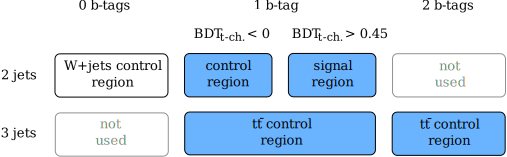
\includegraphics[scale=0.75]{figures/polarization/regions.pdf}
}

\section{Training of Boosted Decision Trees}


%choice of variables, correlation tests

\section{Signal extraction}

\section{W+jet modeling}

\section{Validation}

cosTheta, cosWhel, top mass in SR/CR, 2j0t,3j1t

\section{Unfolding}

bdt cut, neyman construction

\section{Statistical evaluation}

Q-scale reweighting, chi2 fit

\section{Results}

\myfigure{}{
\subfloat[]{\includegraphics[width=0.48\textwidth]{figures/polarization/result/unfolded_mu_top.pdf}}
\hspace{0.02\textwidth}
\subfloat[]{\includegraphics[width=0.48\textwidth]{figures/polarization/result/unfolded_mu_antitop.pdf}}\\
\subfloat[]{\includegraphics[width=0.48\textwidth]{figures/polarization/result/unfolded_mu.pdf}}
}

\section{Limits on anomalous couplings}

topfit
%\chapter{Differential single-top-quark cross sections at 13~TeV}

\section{BDT training}
\label{sec:diff13-bdt}
%\chapter{Conclusion}
\label{ch:conclusion}

polarization:
wp optimization, 2bin unfolding, q scale
eft limits

differential:
extended fitting

%\cleardoublepage
%\appendix % do not forget - otherwise toc messed up!
%\renewcommand{\chaptername}{Appendix}
%\renewcommand\thechapter{\Alph{chapter}}
%\setcounter{chapter}{0}
%\appendixchapter{More on top quarks}

%##############################################
\section{Polarization in top quark pair production}
%##############################################


Similar to the study of the $\mathrm{W}$ boson helicity fractions in top quark decays, the polarization of the top quarks arising in pair production can be analyzed by decomposing the \ttbar cross section as a function of the polarization angles. One finds

\begin{align}
\frac{\mathrm{d}^{2}\sigma}{\sigma\cdot\mathrm{d}\cos\theta_{\mathrm{t}X}^\star~\mathrm{d}\cos\theta_{\bar{\mathrm{t}}X^\prime}^\star}=\frac{1}{4}\Big(1&+\mathrm{P}_\mathrm{t}\,\alpha_{X}\,\cos\theta_{\mathrm{t}X}^\star+\mathrm{P}_{\bar{\mathrm{t}}}\,\alpha_{X^\prime}\,\cos\theta_{\bar{\mathrm{t}}X^\prime}^\star \nonumber \\
&-\mathrm{C}\,\alpha_{X}\alpha_{X^\prime}\,\cos\theta_{\mathrm{t}X}^\star \cos\theta_{\bar{\mathrm{t}}X^\prime}^\star\Big) \label{eq:theory-ttbar-correlation}
\end{align}

where $\mathrm{P}_\mathrm{t}$ and $\mathrm{P}_{\bar{\mathrm{t}}}$ denote the polarization fractions and $\mathrm{C}$ the $\mathrm{t\bar{t}}$ spin correlation. In the helicity basis, the angles are taken between the momenta of the leptons~($X=\ell^{\rmplus}\,/\,X^\prime=\ell^{\rmminus}$) in the corresponding $\mathrm{t}/\bar{\mathrm{t}}$ rest frames and the momenta of the $\mathrm{t}/\bar{\mathrm{t}}$ in the $\ttbar$ \gls{zmf} respectively. Since the top quarks are produced isotropic at \gls{lo}, only a small net polarization of $\mathrm{P}_\mathrm{t}=-\mathrm{P}_{\bar{\mathrm{t}}}\approx0.3\%$ for $m_\mathrm{t\bar{t}}>2m_\mathrm{t}$ from electroweak higher order corrections is expected~\cite{Bernreuther:2010ny,Bernreuther:2013aga}. However, the spins of two top quarks within a pair are linked through the $\mathrm{g\mathrm{t}\bar{\mathrm{t}}}$ vertex yielding a large correlation between them~\cite{Mahlon:2010gw}. The correlation depends on the boost of the top quarks with respect to their \gls{zmf} and amounts to $C\approx32\%$ for $m_\mathrm{t\bar{t}}>2m_\mathrm{t}$ at $8~\TeV$~\cite{Bernreuther:2013aga}. Experimentally, the azimuthal $\Delta\phi$ angle between the two leptons in the laboratory frame is sometimes studied instead of the helicity angle. This observable has the advantage that the whole \ttbar system does not need to be reconstructed which involves finding solutions for the two unknown neutrino momenta while matching the two jets with the two leptons to setup two top quark decay chains\footnote{Kinematic fitting is sometimes deployed to solve this problem using the invariant mass of the intermediate top quarks and $\mathrm{W}$~bosons as constraints.}. The amount of correlation cannot be easily extracted from the $\Delta\phi$ distribution directly since its functional form does not resemble Eq.~\ref{eq:theory-ttbar-correlation}. However this observable is sensitive enough to test the presence of \ttbar correlation and to distinguish it from a potential \gls{bsm} scenario without correlation.


%##############################################
\section{Mass definitions}
%##############################################

Quarks cannot be observed freely at low energies because of strong interactions. Hence, the concept of mass for a quark needs to be defined through renormalization. The top quark is however special since it can be treated as a nearly free particle around and beyond the electroweak energy scale. This leads to two common definitions of its mass which are described in the following. It is important to know which definition is used when comparing theoretical predictions to experimental data or even attempting to infer the ``mass'' from data itself.

The general problem arises from higher order corrections to the ``bare'' quark propagator as depicted in Fig.~\ref{fig:theory-quark-selfenergy}. 

\myfigure{\label{fig:theory-quark-selfenergy}Feynman diagrams at \gls{lo} and beyond contributing to the quark propagator.}{
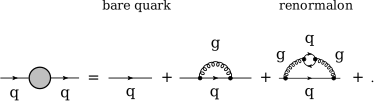
\includegraphics[scale=0.75]{figures/theory/quark_selfenergy.pdf}
}

These result in corrections which are absorbed into the mass definition using the concept of renormalization. The procedure is similar to the running strong coupling constant as briefly described in Sec.~\ref{sec:theory-qcd}. The ``bare'' quark propagator is modified after renormalization as

\begin{equation}
\frac{i}{\gamma_{\mu}p^{\mu}-m_\mathrm{bare}}\quad\Rightarrow\quad\frac{i}{\gamma_{\mu}p^{\mu}-m_\mathrm{bare}+\Sigma(p,m_\mathrm{bare},\mu)}
\end{equation}

where $m_\mathrm{bare}$ denotes the bare mass of a quark which is however unphysical and just a parameter in the Lagrangian. The function $\Sigma(p,m_\mathrm{bare},\mu)$ is called ``self-energy'' and contains finite corrections but also divergent terms where the later arise from the used regularization procedure\footnote{Dimensional regularization with $\epsilon=(4-d)/2$ leads to counterterms with $1/\epsilon$ divergences.}. It depends on the renormalization scale $\mu$ beyond which higher order corrections have been absorbed.

For the top quark, a common scheme is the on-shell renormalization. Here, one requires $\Sigma(p)=0$ and $\mathrm{d}\Sigma/\mathrm{d}p=0$ for $p=m$ which defines $m$ as the pole mass. However, this scheme is normally only suited for particles which are free at low energies like the leptons. For the top quark, an additional problem in the calculation of the self-energy arises from special diagrams called ``renormalons'' which feature vacuum polarization bubbles~(see last diagram in Fig.~\ref{fig:theory-quark-selfenergy}). These lead to an ambiguity on the order of $\Lambda_\mathrm{QCD}\approx200~\MeV$ in the top-quark pole mass definition\footnote{Technically, this ambiguity stems from the chosen path of integration around the singularities from the renormalons~\cite{Smith:1996xz}.}. Despite this, one usually refers to the pole mass as the top quark mass which is also adopted in this thesis. However, since this level of precision is nearly approached in measurements of the top quark mass, the ambiguity has to be understood further or one should move to other schemes instead~\cite{Smith:1996xz}.

The other common renormalization scheme is the \glsreset{msbar}\gls{msbar}. Here, only the divergent terms within the self-energy are absorbed into the mass definition. The mass will therefore depend explicitly on the renormalization scale. However, this allows to define also the mass of quarks at very low energies. In literature, this scheme is commonly used for the light quarks~\cite{Olive:2016xmw}. For the top quark, a difference of

\begin{equation}
m_\mathrm{pole}^\mathrm{t}-m_{\gls{msbar}}^\mathrm{t}(\mu)=173.5~\GeV-163.1~\GeV=10.4~\GeV
\end{equation}

has been calculated at \gls{nnlo} in \gls{qcd} between the pole and \gls{msbar} mass definitions for $\mu=m_\mathrm{pole}$~\cite{Jegerlehner:2012kn}.

In conclusion, it should be stressed that the top quark mass is not an observable. Measuring the top quark mass requires to use experimental observables like (differential) cross sections to infer the top quark mass by comparing data to theoretical calculation for different masses and definitions. 


%\appendixchapter{Track reconstruction in the CMS FastSimulation package}

\intro{Simulated samples of events are a key ingredient within analyses for understanding the detector and the physics behind \gls{lhc} collision data. An introduction to the FastSimulation (\gls{fsim}) package of \gls{cms} is given in this chapter. It provides a fast alternative for simulating the detector response and emulating the reconstruction of events compared to the standard simulation and reconstruction workflow of \gls{cms}. This is achieved by replacing some computing-intense parts in the standard simulation and reconstruction chain with various approximations. One particular speedup is obtained by using an own track reconstruction which relies on truth information to solve the combinatorial problem of associating reconstructed hits to trajectories. In addition, details about the generation of reconstructed hits in the inner tracking system and the seeding of trajectory in \gls{fsim} are given. Before the chapter is concluded the performance of the emulated track reconstruction is validated. This chapter is mostly based on Ref.~\cite{fastsim-mkomm}.}

\todo{update ref when proceedings accepted}


%##############################################
\section{Introduction}
%##############################################

Simulating the detector response for arbitrary events is of crucial importance for understanding recorded collision data and to infer properties of the underlying physics in analyses. The standard package for simulation collision events in \gls{cms} is called ``FullSimulation''~\cite{1742-6596-396-2-022003,1742-6596-664-7-072022}. It is based on the \GEANT{}4 toolkit~\cite{Agostinelli2003250} and provides a detailed simulation of the detector response and an emulation of its readout systems. Simulated events are reconstructed utilizing the same event reconstruction algorithms as utilized for data.

A fast alternative to the standard simulation and reconstruction workflow is provided by the ``FastSimulation'' (\FSIM[format=hyperbf]) package of \gls{cms}. It delivers high-level analysis objects with sufficient accuracy for analyses while being tightly integrated into the \gls{cms} software framework~\cite{Bayatian:922757} along the standard simulation and reconstruction workflow. Its simulation speed of less than 10~s per event\footnote{For events with up to $\approx30$ pileup interactions on average.} is achieved by sidestepping certain parts in the standard simulation and reconstruction chain and utilizing various approximations instead. The two major CPU-intense parts which are replaced are the \GEANT{}4-based~\cite{Agostinelli2003250} simulation of particle interactions with the detector material and the track reconstruction. In particular, the complex, multistep algorithms which reconstruct tracks from energy depositions left by traversing charged particles in the \gls{cms} inner tracking system are exchanged with simpler versions that rely on truth-information about the simulated events. The final analysis objects produced by \FSIM are indistinguishable from the ones produced by the standard simulation and reconstruction workflow. This enables an easy integration of \FSIM samples in analyses along standard simulation and data samples.

Nowadays, the \FSIM package is successfully employed within \gls{cms} analyses. Typical use cases are searches for \acrfull{bsm} physics like \acrfull{susy}. These analyses require usually multiple signal samples which reflect various realizations of a new physics model. Other use cases are the evaluation of the impact of systematic uncertainties on a measurement like a variation of the renormalization and factorization scales or the top quark mass. A more general use case is to increase the statistics of existing samples for training \acrfull{mva} methods. The development of \FSIM is further motivated in the light of increasing luminosity and data statistics for which larger samples of simulated events with higher pileup conditions have to be produced for analysis.

In this chapter the \FSIM package is introduced with an emphasis on the employed track reconstruction for simulated events as follows. First an overview of the standard simulation and the specialized \FSIM workflows are given in Sec.~\ref{sec:fsim-workflow}. Then, the generation of reconstructed hits (Sec.~\ref{sec:fsim-hits}) and the emulation of the iterative track reconstruction are detailed (Sec.~\ref{sec:fsim-tracking}) where the latter focuses in particular on the seeding of trajectories for initiating the iterative tracking sequence. A validation of the track reconstruction is presented in Sec.~\ref{sec:fsim-validation} where the obtain performances are compared with the result of the standard simulation and reconstruction. The chapter is concluded in Sec.~\ref{sec:fsim-conclusion}.


%##############################################
\section{Simulation workflow}
%##############################################
\label{sec:fsim-workflow}

The individual steps within the \gls{cms} software to obtain simulated events for comparison with data are sketched in the following with an emphasis on the differences between the standard and \FSIM workflows.

\begin{description}
\item[Generation] The sample generation commences by creating collections of particles with the help of \acrfull{mc} generators that are configured to produce events according to some physics process of interest. This step can also be performed independently of the core \gls{cms} software. Common interfaces with generator programs are provided through the \HEPMC[format=hyperbf]~\cite{Dobbs:2001ck} or \LHEF[format=hyperbf]~\cite{Alwall:2006yp} event formats.

\item[Simulation] The trajectories of the generated particles are propagated through a geometrical model of the detector starting from the interaction point. As the particles traverse the detector, their interaction with the encountered material is simulated. In the standard simulation, the \GEANT{}4 package is utilized which provides a detailed propagation of particles in the magnetic field and a sophisticated simulation of the various interactions. 
In \FSIM a simplified detector geometry is utilized for the inner tracking system. Interactions are only simulated on infinitely thin cylindrical layers and endcap disks using parameterized models for energy loss through ionization, bremsstrahlung, photon conversion, and multiple scattering. Since a constant magnetic field is assumed as well the propagation of particles between the layers is performed analytically. In a final step the intersection points of the trajectories with the simplified geometry are projected onto the real geometry of the tracking system to create simulated hits associated to actual tracker modules. In the calorimetry systems \gls{em} or hadronic showers are simulated by sampling energy deposits from parameterized models of the expected longitudinal and transverse shower profiles per particle type and energy.

\item[Digitalization] An emulation of the detector readout systems is performed in the digitalization step. After this stage, the event record in the standard simulation contains similar information as found in recorded raw data events. In \FSIM the digitalization algorithms of the standard simulation workflow are also utilized for the calorimeter systems. For the tracker hits no detailed simulation of the charge deposition is performed. Instead, the reconstruction of hits from charge clusters is only emulated by performing a smearing of the simulated hit positions are detailed in Sec.~\ref{sec:fsim-hits} below.

\item[Reconstruction] In \FSIM the standard event reconstruction is applied to simulated events as well with the exception of the track reconstruction. Here, the computing-intense tracking algorithm with includes amongst others the \acrfull{ctf} algorithm~\cite{Chatrchyan:2014fea} are bypassed by utilizing truth-information about the simulated events instead to solve the combinatorial problem.
\end{description}

The tight integration of the \FSIM package within the \gls{cms} software allows to utilize most of the standard data containers within its workflow so that simulated \FSIM samples can easily be used by analysts along samples generated with the standard event simulation and reconstructed data. 


%##############################################
\section{Emulation of hit reconstruction}
%##############################################
\label{sec:fsim-hits}

An emulation of the local hit reconstruction for the tracker modules has to be performed since no detailed information of charge deposition is generated in the simulation step of \FSIM. To mimic the resolutions of the standard hit reconstruction the true hit positions are smeared. A new \FSIM module for position smearing has been developed which allows to manage various algorithms for position smearing side-by-side. It can be flexibly configured for any topology of the tracker. Additionally, each algorithm can be restricted to certain tracker modules only. A sketch of the inner workings of the new module is shown in Fig.~\ref{fig:fsim-hitsmearing}.

\myfigure{\label{fig:fsim-hitsmearing}Emulation of local hit reconstruction in \FSIM.  Various algorithm can be configured side-by-side. A flexible selection syntax allows to specify on a per module basis which hits to process.}{
\includegraphics[scale=0.75]{figures/fastsim/parcels.pdf}
}

First, the simulated hits are sorted according the associated tracker module. Then, algorithms for hit position smearing are loaded dynamically based on a configuration that is supplied by the user. Each instance of an algorithm can be configured to select and process only hits belonging to certain tracker modules. The selection is achieved through a special syntax parser for evaluating the user configuration dynamically against the module properties. Technically, the \texttt{Boost.Spirit} framework~\cite{boostspirit} is utilized to implement the parser based on grammar rules written in \glshere{ebnf}. This allows to extended the syntax easily in case of future requirements that are at the moment uncovered.

Currently, a simple Gaussian smearing of the position is employed for all strip modules where the configured resolution depends on the specific tracker subdetector (\gls{tib}, \gls{tid}, \gls{tob}, \gls{tec}) and its layer. A more detailed emulation of hit reconstruction is performed for the pixel modules where parametrized distributions from the standard template-based hit reconstruction are utilized for the smearing. These templates are generated using the \texttt{PixelAV} program which simulates the distributions of charges in pixel modules while accounting for their Lorentz drift in the magnetic field and potential radiation damage of the sensor~\cite{Swartz:2002kda}. The new \FSIM module allows furthermore the emulation of producing merged hits which occur in data when the distributions of the deposited charges from two particles transversing a tracker module overlap. Figure~\ref{fig:fsim-merge} shows a recent study of the probability of hit merging on the pixel modules. Such probability maps are expected to be used for the emulation of hit merging in the future.


\myfigure{\label{fig:fsim-merge}Probability of two hits merging on the pixel barrel modules as a function of their distance and local incident angle of a track expressed in pseudorapidity.}{
\includegraphics[width=0.48\textwidth]{figures/fastsim/merge.pdf}
}




%##############################################
\section{Emulation of track reconstruction}
%##############################################
\label{sec:fsim-tracking}

In \FSIM an emulation of the iterative track reconstruction is performed. The sequence of seeding, trajectory building and fitting and the iterative steps are kept similar to the standard track reconstruction but all algorithms are replaced with \FSIM-specific versions. A central idea to speedup the track reconstruction in \FSIM is to solve the combinatorial problem of associating reconstructed hits to particle trajectories by using \gls{mc}-truth information. An overview of the idea is shown in Fig.~\ref{fig:fsim-tracking}. Starting from a collection containing all reconstructed hits, each hit is mapped back to the simulated track from which it originated in the simulation. Then, the iterative tracking is carried out where each step is performed multiple times per subset of hits that belong to a single simulated track. This approach circumvents entirely any combinatorial confusion of hits. Thus, no fake tracks from a combination of spurious hits are emulated and the resulting tracking efficiency would in principle be 100\%. However, by accounting for dedicated selection criteria that are specified for each iteration in the standard reconstruction, the efficiency is decreased and becomes comparable to the one obtained in the standard track reconstruction as demonstrated in Sec.~\ref{sec:fsim-validation} below.

\myfigure{\label{fig:fsim-tracking}The track reconstruction workflow in \FSIM. Details are given in the text.}{
\includegraphics[scale=0.75]{figures/fastsim/tracking.pdf}
}

The ability to produce merged hits originating from close particle tracks necessitated a recent extension of the \FSIM{}-specific data containers within the iterative tracking sequence. Instead of a one-to-one mapping of reconstructed hits to simulated tracks, close simulated hits can now result into a single reconstructed ``merged'' hit that can be shared between the final tracks within an iteration as indicated in Fig.~\ref{fig:fsim-tracking}. A further benefit of the extension is that the mapping itself can be generated independently from the simulated track information which will allow the mix-in of wrong hit combinations leading to ``fake'' tracks in the future which is currently not emulated.


%##############################################
\subsection{New seeding algorithm}
%##############################################
\label{sec:fsim-seeding}

An algorithm has been developed to identify potential trajectory seed candidates while operating on an arbitrary number of seeding layers efficiently. In the original implementation, only doublets or triplets of hits could act as seeds. However, after the upgrade of the \gls{cms} pixel detector~\cite{Dominguez:1481838} a mixture of doublets, triplets, and quartets are utilized for seeding. This is solved in \FSIM by organizing the seeding layer configuration into a tree-like structure. For example the triplet configurations listed in Tab.~\ref{tab:fsim-seedinglist} can be transformed into the tree-structure as shown in Fig.~\ref{fig:fsim-seedingtree}. The new algorithm commences by iterating over a list of hits and linking them to a corresponding node in the tree. While the tree is being populated, dedicated seed selection criteria are evaluated on already found subsets of hits by interfacing directly with the standard track reconstruction. The exact selection is iteration-dependent and consists of various criteria such as the compatibility of the extrapolated trajectory with the beam spot or primary vertices\footnote{Preliminary primary vertices are reconstructed from tracks found in previous iterations.}. If hits at each node between the root and one of the leafs are found that are also compatible with any corresponding selection criteria the algorithm is stopped and the found seed candidate passed to the subsequent trajectory building and fitting stages as shown in Fig.~\ref{fig:fsim-tracking}.

\mytable{\label{tab:fsim-seedinglist}Exemplary configurations of pixel barrel (\gls{bpx}) and pixel forward (\gls{fpx}) layers where trajectory seed candidates can be generated from hits.}{
\begin{tabular}{@{}l l@{\,}l l@{\,}l l@{\,}l l@{\,}l l@{\,}l@{}}
\toprule
 & \multicolumn{10}{c}{Triplet layers} \\
First hit & BPX&1 & BPX&1 & BPX&1 & BPX&1 & BPX&1 \\
Second hit & BPX&2 & BPX&2 & BPX&2 & FPX+&1 & FPX-&1 \\
Third hit & BPX&3 & FPX+&1 & FPX-&1 & FPX+&2 & FPX-&2 \\
\bottomrule
\end{tabular}
}

\myfigure{\label{fig:fsim-seedingtree}Exemplary configurations of pixel barrel (\gls{bpx}) and pixel forward (\gls{fpx}) layers where trajectory seed candidates can be generated from hits. A seed has to contain corresponding hits at each node between the root and one of the leafs.}{
\includegraphics[scale=0.75]{figures/fastsim/seedingtree.pdf}
}

The developed tree-structure allows to performed seed generation from an arbitrary number of layers without using nested or recursive iterations over the reconstructed hits which makes it also fairly efficient.

%##############################################
\section{Validation}
%##############################################
\label{sec:fsim-validation}

The track reconstruction within \FSIM is validated by comparing the produced tracks with those obtained from the standard simulation and reconstruction workflow. A comparison of the resulting tracking efficiency as a function of the transverse momentum and pseudorapidity is presented in Fig.~\ref{fig:fsim-eff-tracks}, where the tracking efficiency is defined as the ratio of reconstructed tracks matched to simulated charged particles over the total number of charged particles within the tracker volume. Furthermore, the obtained resolution of the transverse momentum for reconstructed tracks is shown in Fig.~\ref{fig:fsim-res-track}. Overall, the distributions demonstrate a good agreement of the \FSIM tracking performance with the one obtained from the standard simulation and reconstruction workflow.

\myfigure{\label{fig:fsim-eff-tracks}Comparison of the reconstruction efficiencies of tracks as a function of (a)~the transverse momentum and (b)~the pseudorapidity measured in the simulation of top quark pair production at 13~TeV.}{
\subfloat[]{\centering\includegraphics[width=0.48\textwidth]{figures/fastsim/eff_pt.pdf}}
\hspace{0.02\textwidth}
\subfloat[]{\centering\includegraphics[width=0.48\textwidth]{figures/fastsim/eff_eta.pdf}}
}

A profile of the average CPU-time consumption per event within \FSIM is given in Fig.~\ref{fig:fsim-cpu} as a function of the average number of pileup interactions. Less than 10~s are required to simulated an event of top quark pair production for current pileup scenarios with $\approx30$ interactions on average. The presented emulation of tracking in this chapter is not amongst the top CPU consumers.

\myfigure{\label{fig:fsim-res-track}Comparison of the resolution of reconstructed tracks as a function of the transverse momentum measured in the simulation of top quark pair production at 13~TeV.}{
\includegraphics[width=0.48\textwidth]{figures/fastsim/res_pt.pdf}
}

\myfigure{\label{fig:fsim-cpu}Average CPU-time per event spent on the detector simulation and the reconstruction of analysis objects as a function of the average number of pileup interactions measured in the simulation of \ttbar production at 13~TeV using the \texttt{IgProf}~\cite{Eulisse:865673} profiler.}{
\includegraphics[width=0.65\textwidth]{figures/fastsim/cpu_profile.pdf}
}

%##############################################
\section{Conclusion}
%##############################################
\label{sec:fsim-conclusion}

The \gls{cms} \FSIM package provides a fast alternative to the standard simulation and reconstruction workflow for generation samples of simulated events. One of its major speedups is the usage of truth information in the track reconstruction. Recent developments in the framework led to further flexibility in the emulation of hit reconstruction and in the iterative tracking sequence. In the short term, these developments will enable the emulation of merged hits originating from close particle tracks. In the long term, the increased flexibility will allow to adapt the emulation of track reconstruction to the (planned) upgrades of the \gls{cms} detector.






\glsaddall[types={acronym}] 
\renewcommand*{\arraystretch}{1.1}
\printglossary[style=super,nopostdot,type=\acronymtype,title={Abbreviations},nonumberlist]
\renewcommand*{\arraystretch}{\mytablestrech}
\cleardoublepage

%\nocite{*}
\bibliographystyle{style/bibstyle}
\renewcommand{\bibname}{References}
\bibliography{sections/references}

\todototoc
\listoftodos

\end{document}
